\documentclass{article}
\usepackage{ amssymb }
\usepackage{amsmath}
\usepackage{mathtools}
\usepackage{tikz}
\usepackage{float}
\usepackage{graphicx}
\usepackage{subcaption}
\usepackage{hyperref}
\usepackage[super]{nth}
\usepackage[margin=0.8in]{geometry}
\newcommand{\norm}[1]{\left\lVert#1\right\rVert}
\usetikzlibrary{patterns}

\title{Numerical methods for Differential equations Report 2}
\author{Malte Wegener (4672194)}
\date{\today}

\begin{document}

\maketitle
\section{Inhomogeneous poisson equation}
In the this section, the following Boundary Value Problem (BVP) will be solved using a Finite volume method.

\begin{equation}
\begin{aligned}-\nabla \cdot(k \nabla u) &=f, \quad(x, y) \in \Omega=(0,8) \times(0,4) \\ u(x, y) &=0, \quad(x, y) \in \partial \Omega \\ k(x, y) &=1+4 x+6 y, \quad(x, y) \in \bar{\Omega} \\ f(x, y) &=e^{\alpha(x-1)^{2}+\alpha(y-1)^{2}}+e^{\alpha(x-3)^{2}+\alpha(y-1)^{2}} \\ &+e^{\alpha(x-1)^{2}+\alpha(y-1)^{2}}+e^{\alpha(x-3)^{2}+\alpha(y-3)^{2}} \\ &+e^{\alpha(x-5)^{2}+\alpha(y-3)^{2}}+e^{\alpha(x-7)^{2}+\alpha(y-3)^{2}} \\ & \text { with } \alpha=-5, \quad(x, y) \in \bar{\Omega} \end{aligned}
\end{equation}

With $\bar{\Omega}=[0,8] \times[0,4]$. In order to discretize the PDE, the following stencil on a doubly uniform grid with step h is considered.
\begin{figure}[H]
	\centering
	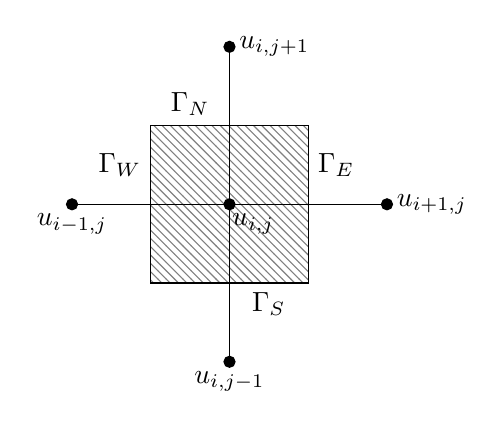
\begin{tikzpicture}
		\draw[pattern=north west lines, pattern color=gray] (-1,-1) rectangle (1,1);
	\draw (1,0.5) node[anchor=west] {$\Gamma_E$};
	\draw (-1,0.5) node[anchor=east] {$\Gamma_W$};
	\draw (-0.5,1) node[anchor=south] {$\Gamma_N$};
	\draw (0.5,-1) node[anchor=north] {$\Gamma_S$};
	
	\filldraw (0,0) circle (2pt);
	\draw (0.3,0) node[anchor=north] {$u_{i,j}$};
	
	\filldraw (-2,0) circle (2pt);
	\draw (-2,0) node[anchor=north] {$u_{i-1,j}$};
	
	\filldraw (2,0) circle (2pt);
	\draw (2,0) node[anchor=west] {$u_{i+1,j}$};
	
	\filldraw (0,-2) circle (2pt);
	\draw (0,-2) node[anchor=north] {$u_{i,j-1}$};
	
	\filldraw (0,2) circle (2pt);
	\draw (0,2) node[anchor=west] {$u_{i,j+1}$};
	
	\draw (-2,0) -- (2,0);
	\draw (0,-2) -- (0,2);
	
	
	\end{tikzpicture}
	\caption{Stencil used for the discretization}
\end{figure} 
In order to discretize the PDE with a finite volume method (FVM), it has to be integrated over a control volume $V_{i,j}$, which is represented by the hatched Area, whose boundary is $\Gamma_{i,j}$.

\begin{equation}
\iint_{V_{i,j}}[-\nabla \cdot(k \nabla u)] d V=\iint_{V_{i,j}} f d V
\end{equation}
Using the Divergence Theorem
\begin{equation}
\oint_{\Gamma_{i,j}}(-k \nabla u \cdot \mathbf{n}) d \Gamma=\iint_{V_{i,j}} f d V
\end{equation}
Which can be rewritten as
\begin{equation}
\oint_{\Gamma_{ijj}}\left(-k \frac{\partial u}{\partial \mathbf{n}}\right) d \Gamma=\iint_{V_{i,j}} f d V
\end{equation}
By splitting the boundary and using a midpoint approximation for the right hand side
\begin{equation}
\int_{\Gamma_{\mathrm{W}}}\left(k\frac{\partial u}{\partial x}\right) d y+\int_{\Gamma_{\mathrm{E}}}\left(-k \frac{\partial u}{\partial x}\right) d y \\ +\int_{\Gamma_{\mathrm{S}}}\left(k\frac{\partial u}{\partial y}\right) d x+\int_{\Gamma_{\mathrm{N}}}\left(-k \frac{\partial u}{\partial y}\right) d x = f_{i,j}h^2
\end{equation}
By approximating $\frac{\partial u}{\partial x}$ and $\frac{\partial u}{\partial y}$ with a central difference formula and using a midpoint approximation for the Integral, a discrete approximation can be found.
\begin{equation}
k_{i-1 / 2, j} \left(u_{i, j}-u_{i-1, j}\right)- k_{i+1 / 2, j} \left(u_{i+1, j}-u_{i, j}\right)+k_{i, j-1 / 2} \left(u_{i, j}-u_{i, j-1}\right)- k_{i, j+1 / 2} \left(u_{i, j+1}-u_{i, j}\right)=h^2 f_{i,j}
\end{equation}
Which can be rearranged to
\begin{equation}
\begin{aligned}
f_{i j}=&-\frac{k_{i-1 / 2, j}}{h^{2}} u_{i-1, j}-\frac{k_{i, j-1 / 2}}{h^{2}} u_{i, j-1}\\
&+\left(\frac{k_{i-1 / 2, j}}{h^{2}}+\frac{k_{i, j-1 / 2}}{h^{2}}+\frac{k_{i+1 / 2, j}}{h^{2}}+\frac{k_{i, j+1 / 2}}{h^{2}}\right) u_{i, j}\\
&-\frac{k_{i+1 / 2, j}}{h^{2}} u_{i+1, j}-\frac{k_{i, j+1 / 2}}{h^{2}} u_{i, j+1}
\end{aligned}
\end{equation}
When assembling a linear system on a lexicographic grid from this equation, a matrix $A\in\mathbb{R}^{(N_x-1)*(N_y-1)\times(N_x-1)*(N_y-1)}$, where $N_x = 8/h$ and $N_y = 4/h$.
This matrix has 5 non-zero diagonals, located on the main diagonal, right next to the main diagonal and offset by $\pm (N_x-1)$. All these diagonals are full, except for the first off diagonals, which have a 0 on every $N_x^{th}$ element. These diagonals can be made, by calculating k for a flattened shifted  grid, which can be trimmed to include the proper coefficients in the matrix, which is implemented in the code.

\begin{figure}[H]
	\begin{subfigure}{.5\textwidth}
		\centering
		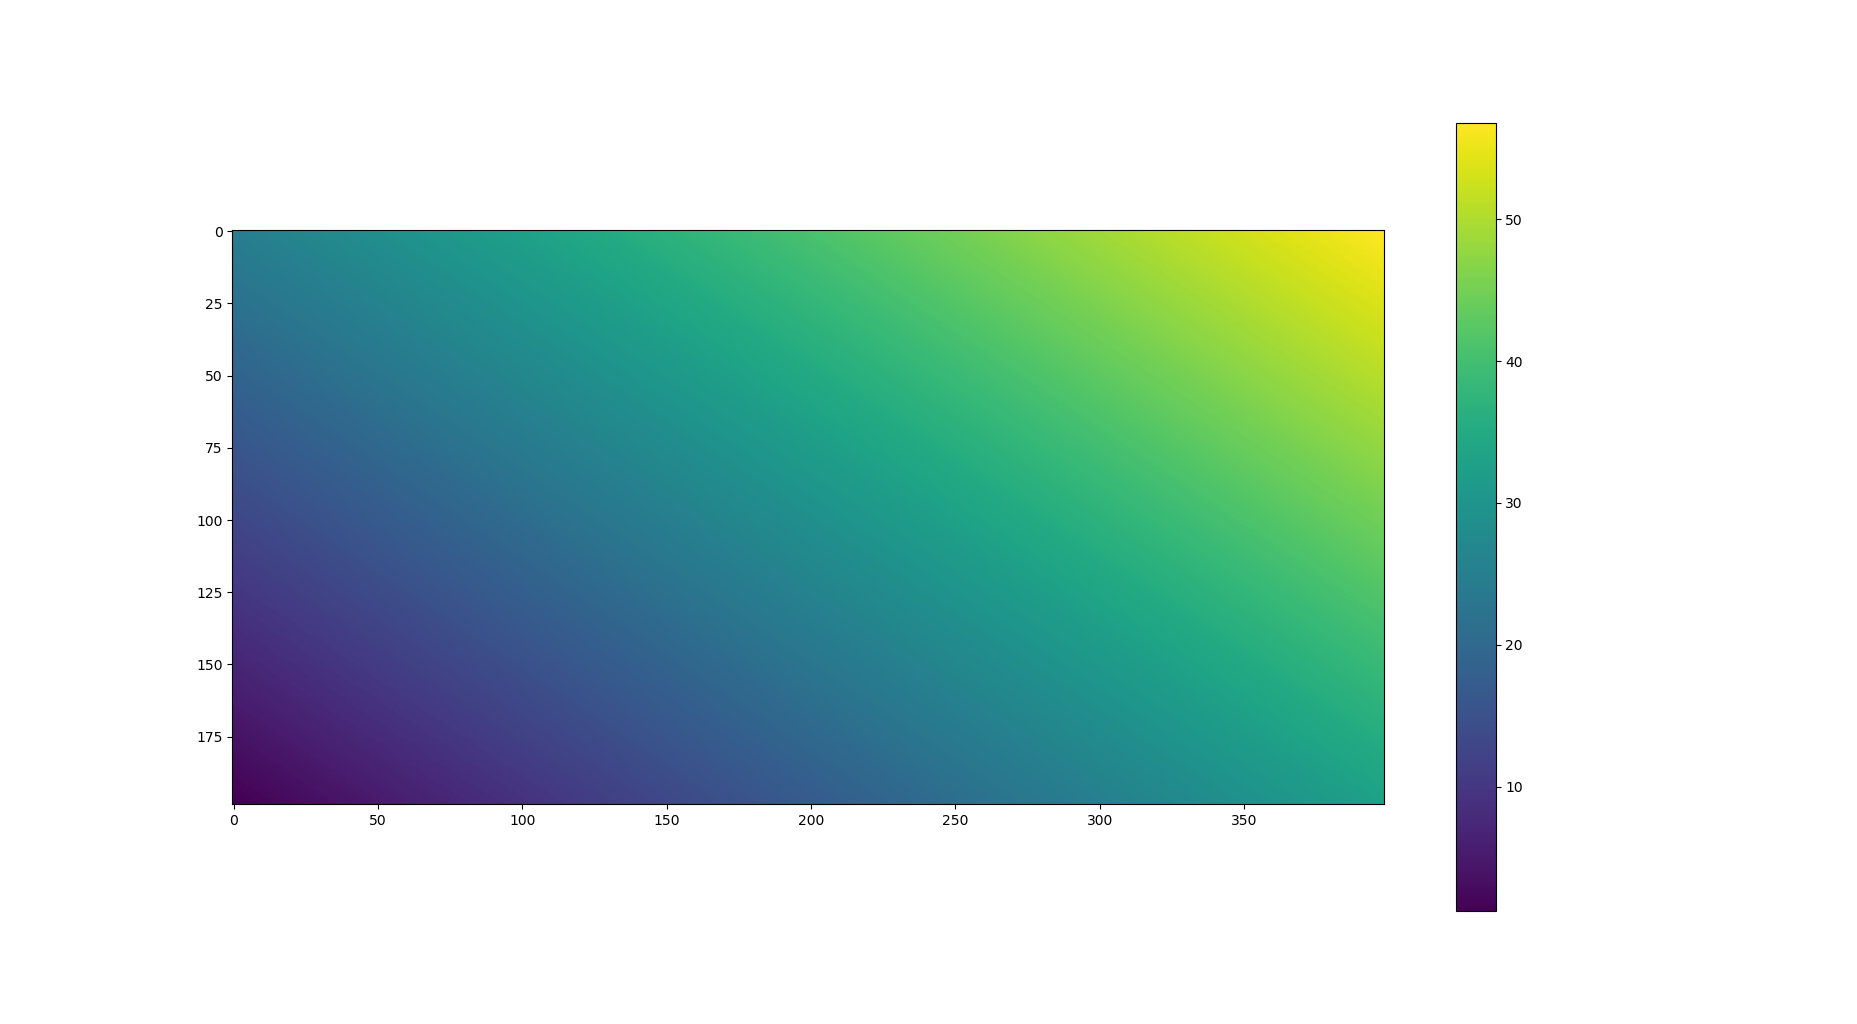
\includegraphics[width=.9\linewidth]{1k.png}
		\subcaption{Coefficient K on the domain}
	\end{subfigure}
	\begin{subfigure}{.5\textwidth}
		\centering
		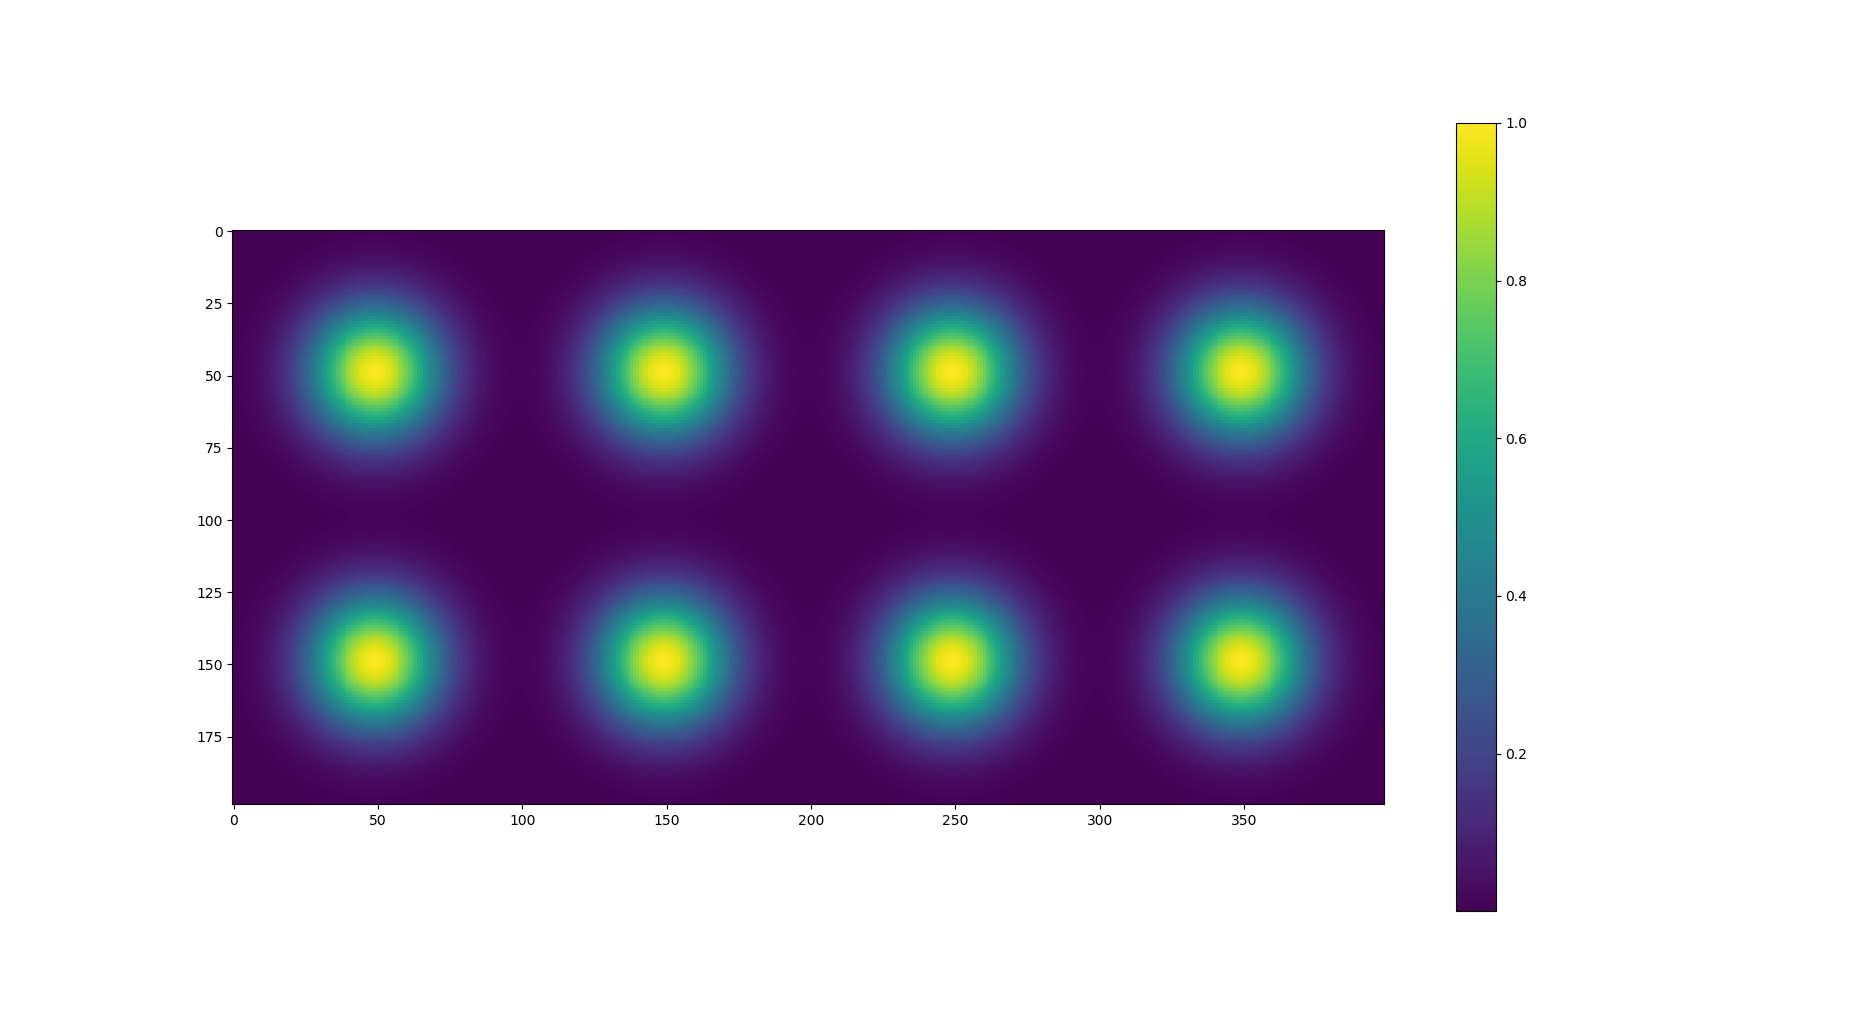
\includegraphics[width=.9\linewidth]{1src.png}
		\subcaption{Source on the domain}
	\end{subfigure}
\end{figure}
\begin{figure}[H]
	\centering
	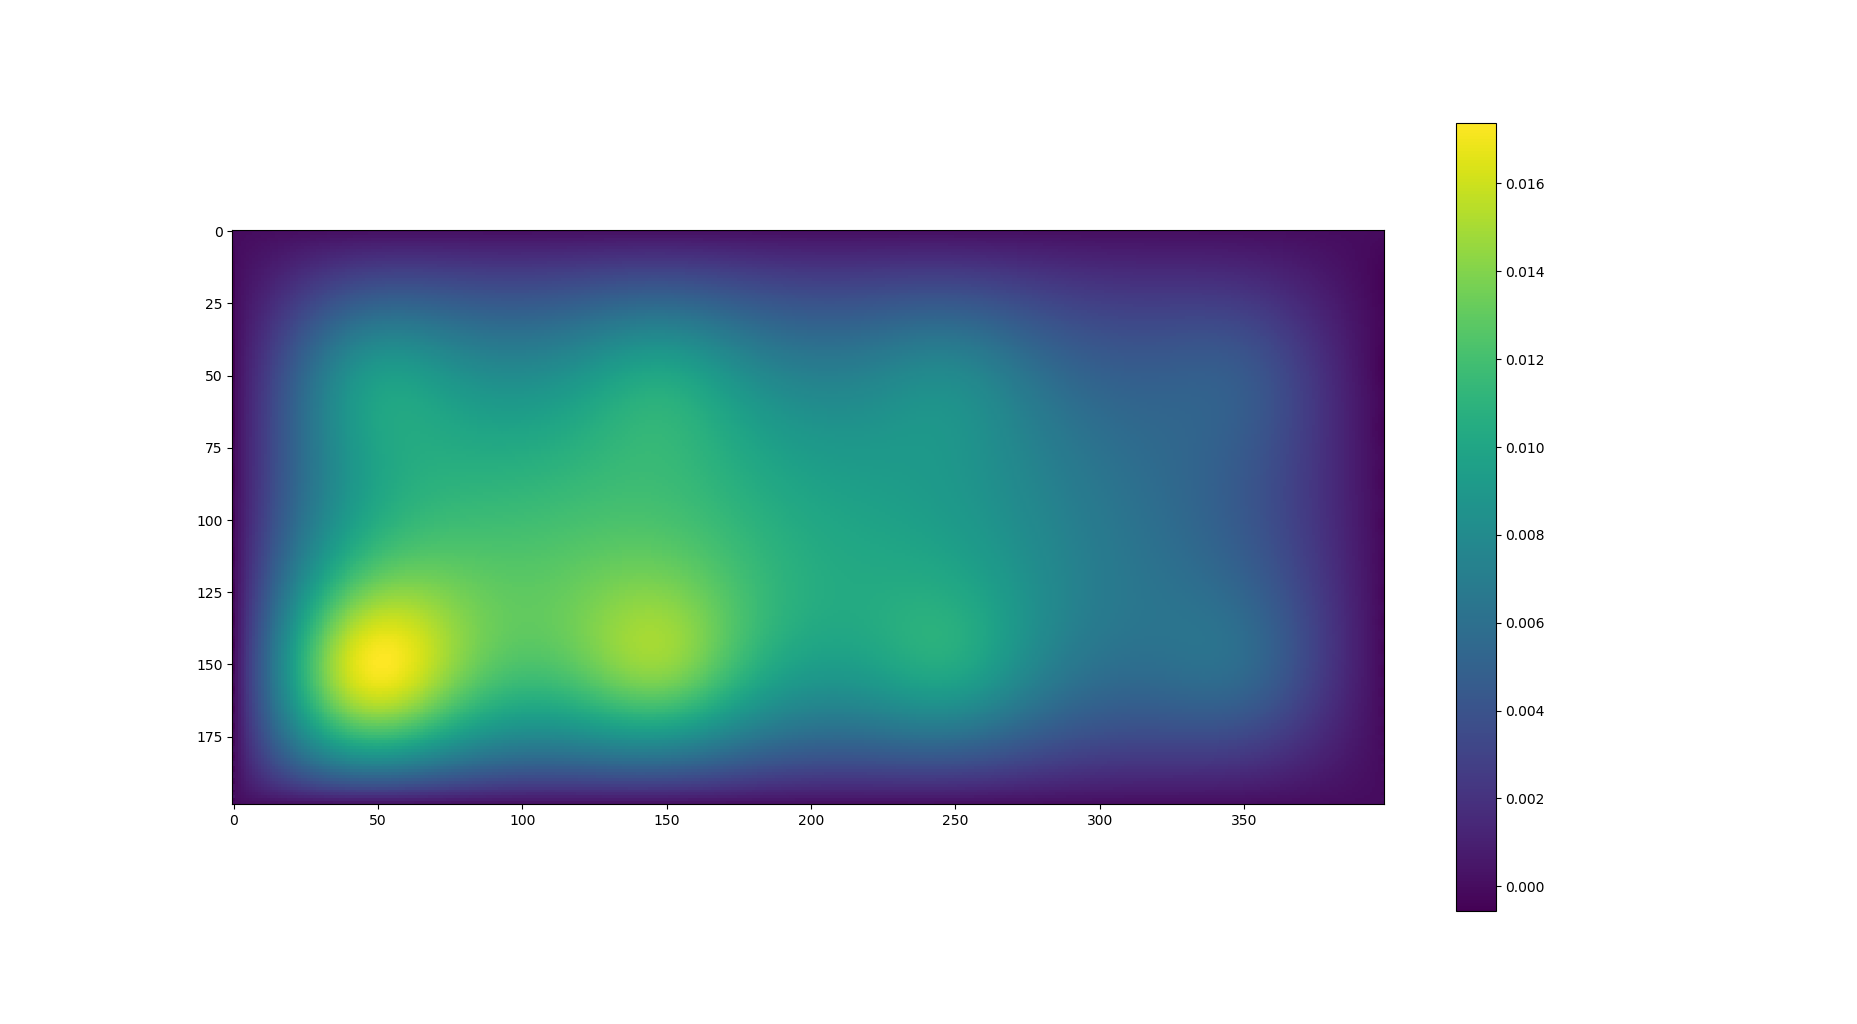
\includegraphics[width=.9\linewidth]{1sol.png}
	\caption{Solution to the BVP on the domain for $h=0.02$}
\end{figure}

The solution seems reasonable, as the source function can be interpreted as a steady influx, that is diffused on the domain. As the rate of diffusion is influenced by k it is expected that the upper right corner will experience stronger diffusion than then the lower left corner, which is the case in the solution. Furthermore, zero Dirichlet boundary conditions are applied, which are also clearly visible in the solution.

\section{Time evolution of the heat equation}
In this section the unsteady heat equation will be solved. This problem can be formulated as the following BVP, with an initial condition.
\begin{equation}
\begin{aligned} \frac{\partial u}{\partial t}-\Delta u=0,\;\;\;\;&(x, y) \in(0,4) \times(0.4), \quad t \in[0,0.15] \\ &u(x, y, t) =0, \quad(x, y) \in \partial \Omega \\ &u(x, y, 0) =e^{\alpha(x-2)^{2}+\alpha(y-2)^{2}} \\ \text { with } &\alpha=-5, (x, y) \in \overline{\Omega} \end{aligned}
\end{equation}
In which $\overline{\Omega} = \left[0,4\right] \times \left[0,4\right]$. This equation can be discretized on a doubly uniform grid with step h. The negative Laplacian in its discrete form can be expressed as $A$, such that the equation becomes
\begin{equation}
\frac{\partial \mathbf{u}}{\partial t}\approx-A\mathbf{u}
\label{eq:sec2approx1}
\end{equation}
In order to solve this unsteady equation, a time-stepping scheme has to be employed. As a simple explicit scheme, Forward Euler (FE) is considered. In this scheme, $\mathbf{u}^{k+1}$ is calculated as
\begin{equation}
\mathbf{u}^{k+1} = \mathbf{u}^{k}+\Delta t*\frac{\partial \mathbf{u}^k}{\partial t}
\end{equation}
By substituting \autoref{eq:sec2approx1}
\begin{align}
\mathbf{u}^{k+1} = \mathbf{u}^{k}-\Delta t*A\mathbf{u}^k\\
\mathbf{u}^{k+1} = (I-\Delta t*A)\mathbf{u}^k
\end{align}
As an implicit method, Backward Euler (BE) is used. $\mathbf{u}^{k+1}$ in BE is calculated as follows.

\begin{equation}
\mathbf{u}^{k+1} = \mathbf{u}^{k}+\Delta t*\frac{\partial \mathbf{u}^{k+1}}{\partial t}
\end{equation}

By substituting \autoref{eq:sec2approx1}
\begin{align}
\mathbf{u}^{k+1} = \mathbf{u}^{k}-\Delta t*A\mathbf{u}^{k+1}\\
\mathbf{u}^{k+1} + \Delta t*A\mathbf{u}^{k+1}= \mathbf{u}^{k}\\
(I+\Delta t*A)\mathbf{u}^{k+1} = \mathbf{u}^k
\end{align}
In order to solve for $\mathbf{u}^{k+1}$ a linear system has to be solved, thus this is an implicit method.

In order to compare these 2 methods, the time evolution is simulate on a grid with $h=0.08$ and $\delta t = 0.015$. 
\begin{figure}[H]
	\centering
	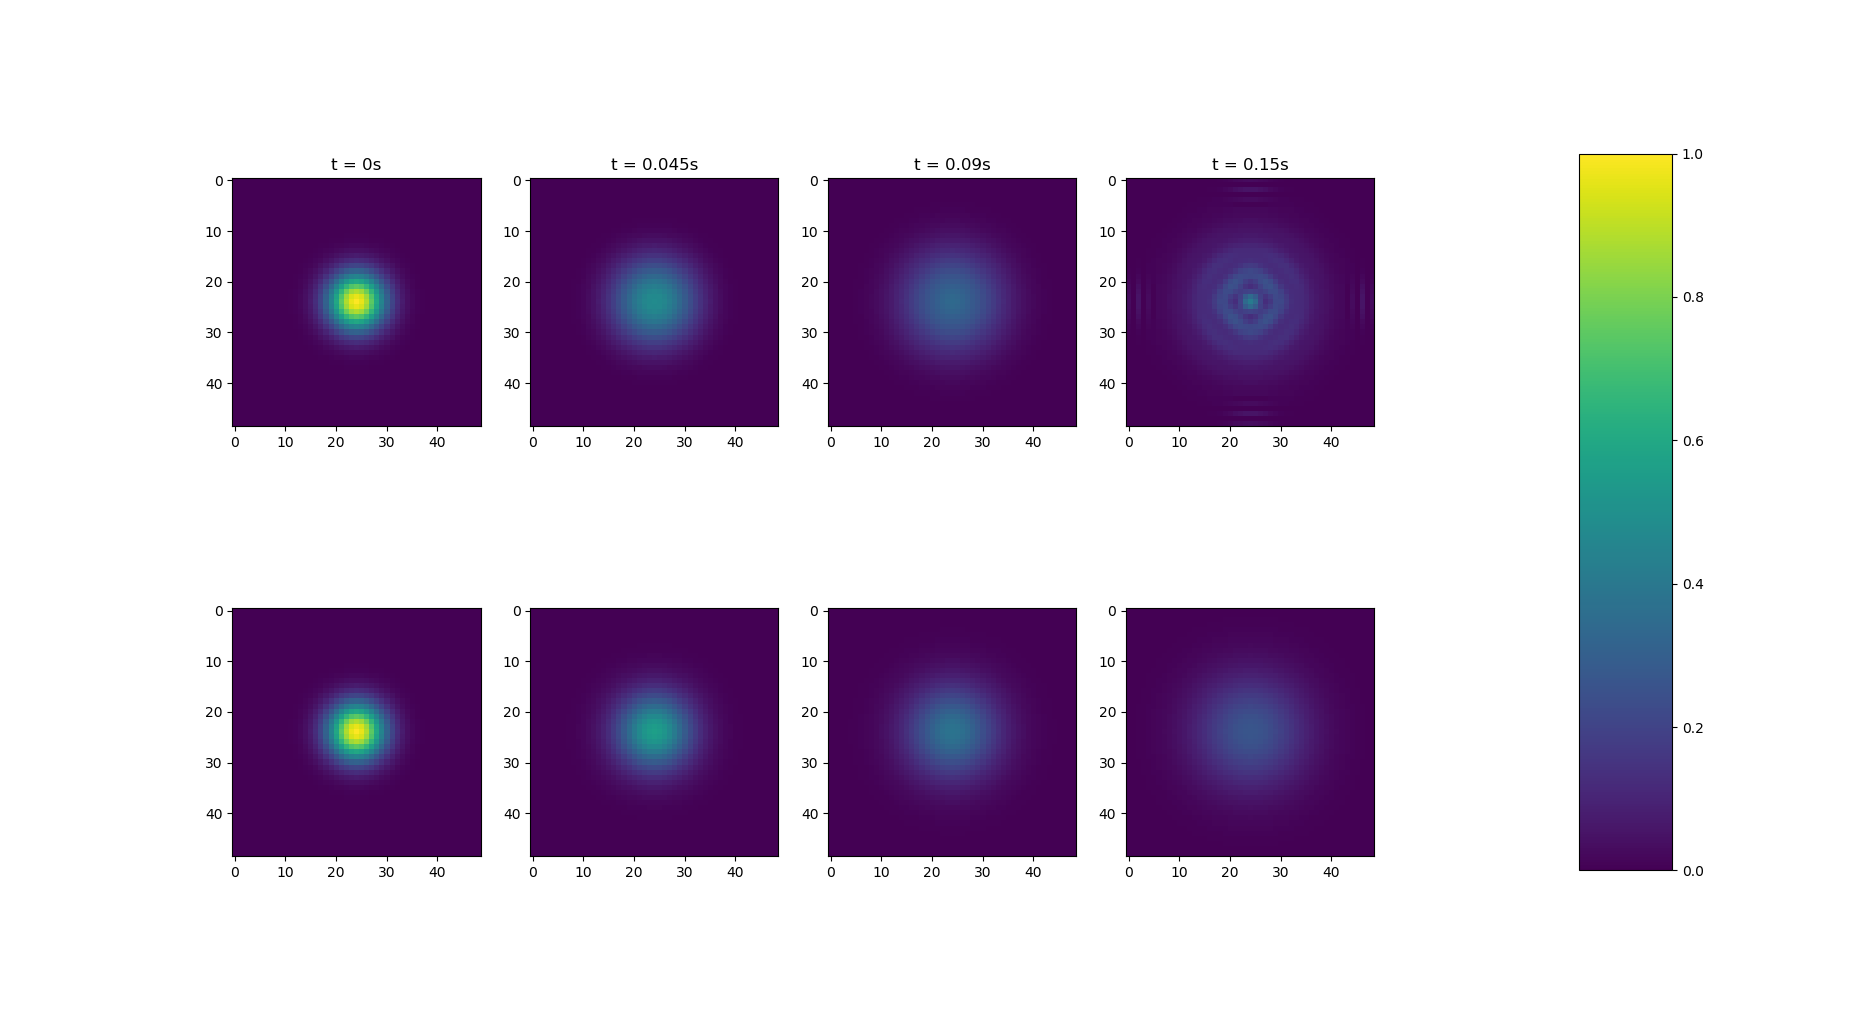
\includegraphics[width=.9\linewidth]{21.png}
	\caption{Time evolution of the Heat equation. First Row presents the Forward Euler, second row is computed with Backwards Euler. All plots are normalized to the same colorscale.}
\end{figure}

It can be seen that FE diffuses faster than BE. Furthermore, FE becomes unstable at $t=0.15$ as the solution does not settle to reach 0 at all points in the domain, which should be expected from the maximum principle.
In order to get stable results from the simulation is run with $\Delta t = 0.005, 0.003 \text{ and } 0.0015$. For $\Delta t = 0.005 \text{and} 0.003$ the solution with FE blows up in the given time, however for $\Delta t = 0.0015$ the solution of FE matches the implicit solution very well.
\begin{figure}[H]
	\begin{subfigure}{.5\textwidth}
		\centering
		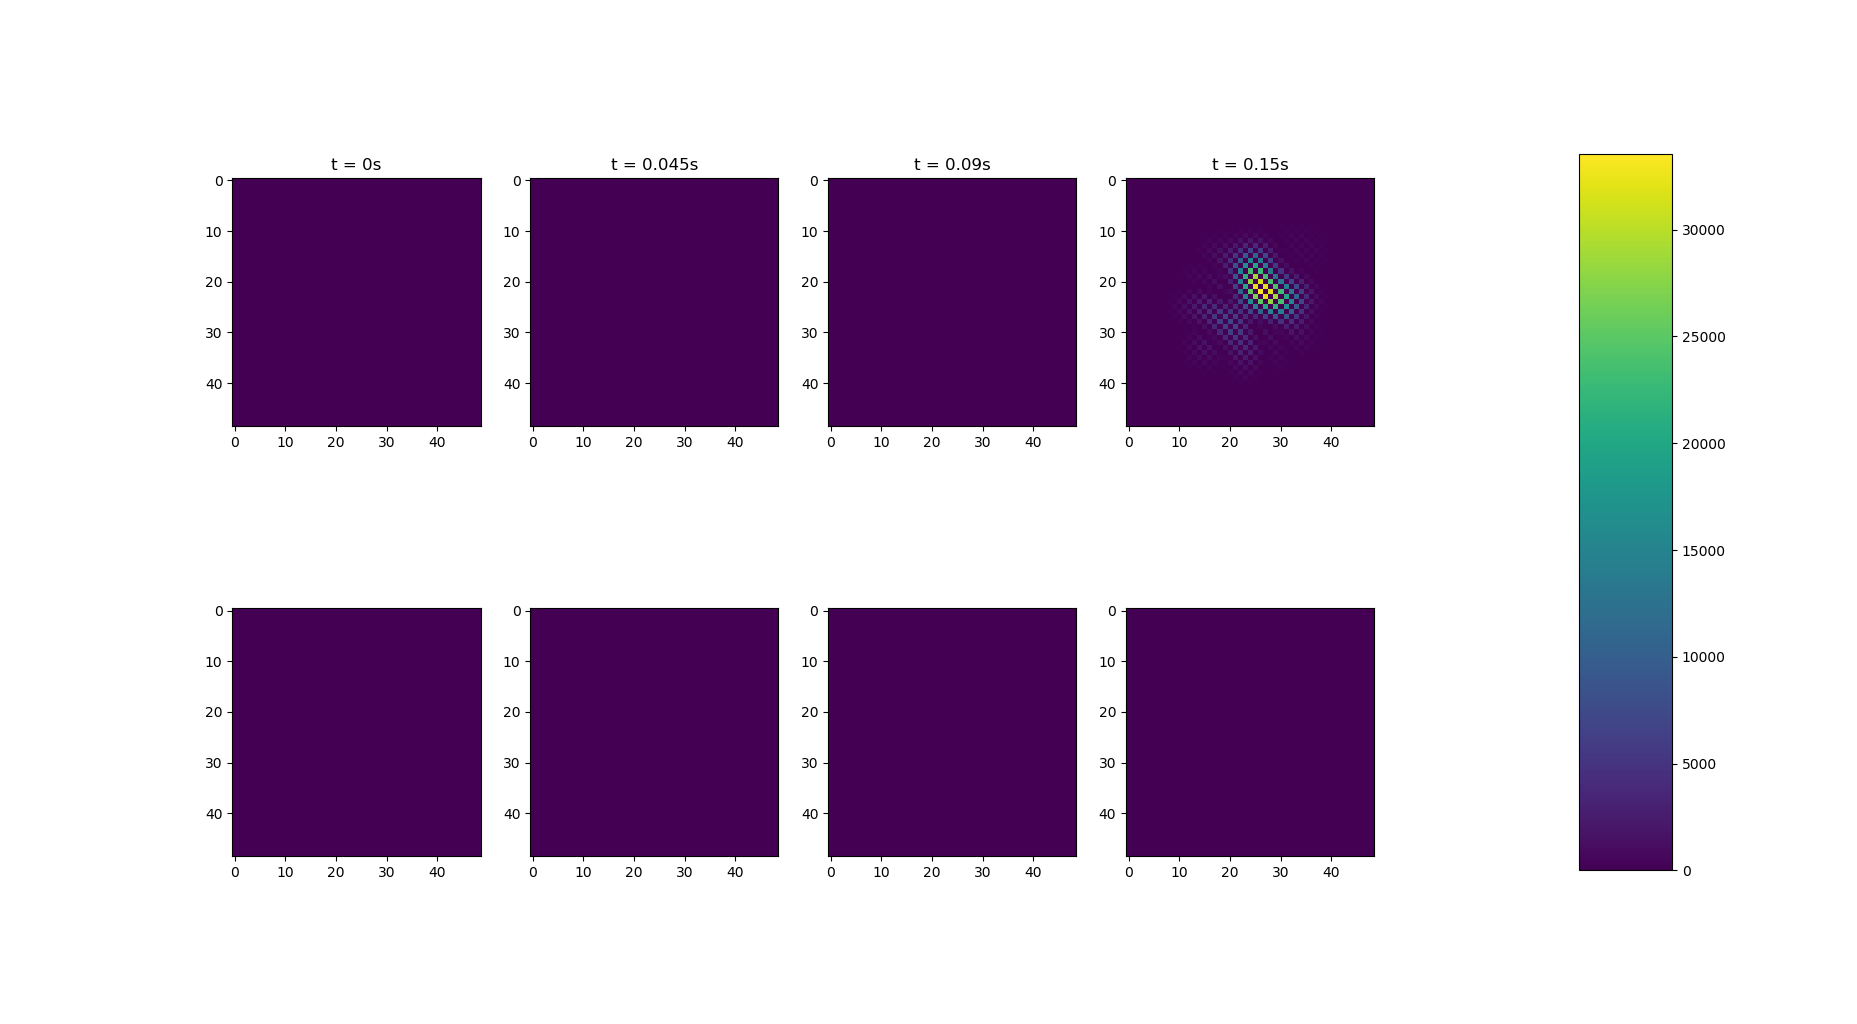
\includegraphics[width=.9\linewidth]{2unstable.png}
		\subcaption{Unstable solution for $\Delta t = 0.005$, with all plots normalized to the same scale}
	\end{subfigure}
	\begin{subfigure}{.5\textwidth}
		\centering
		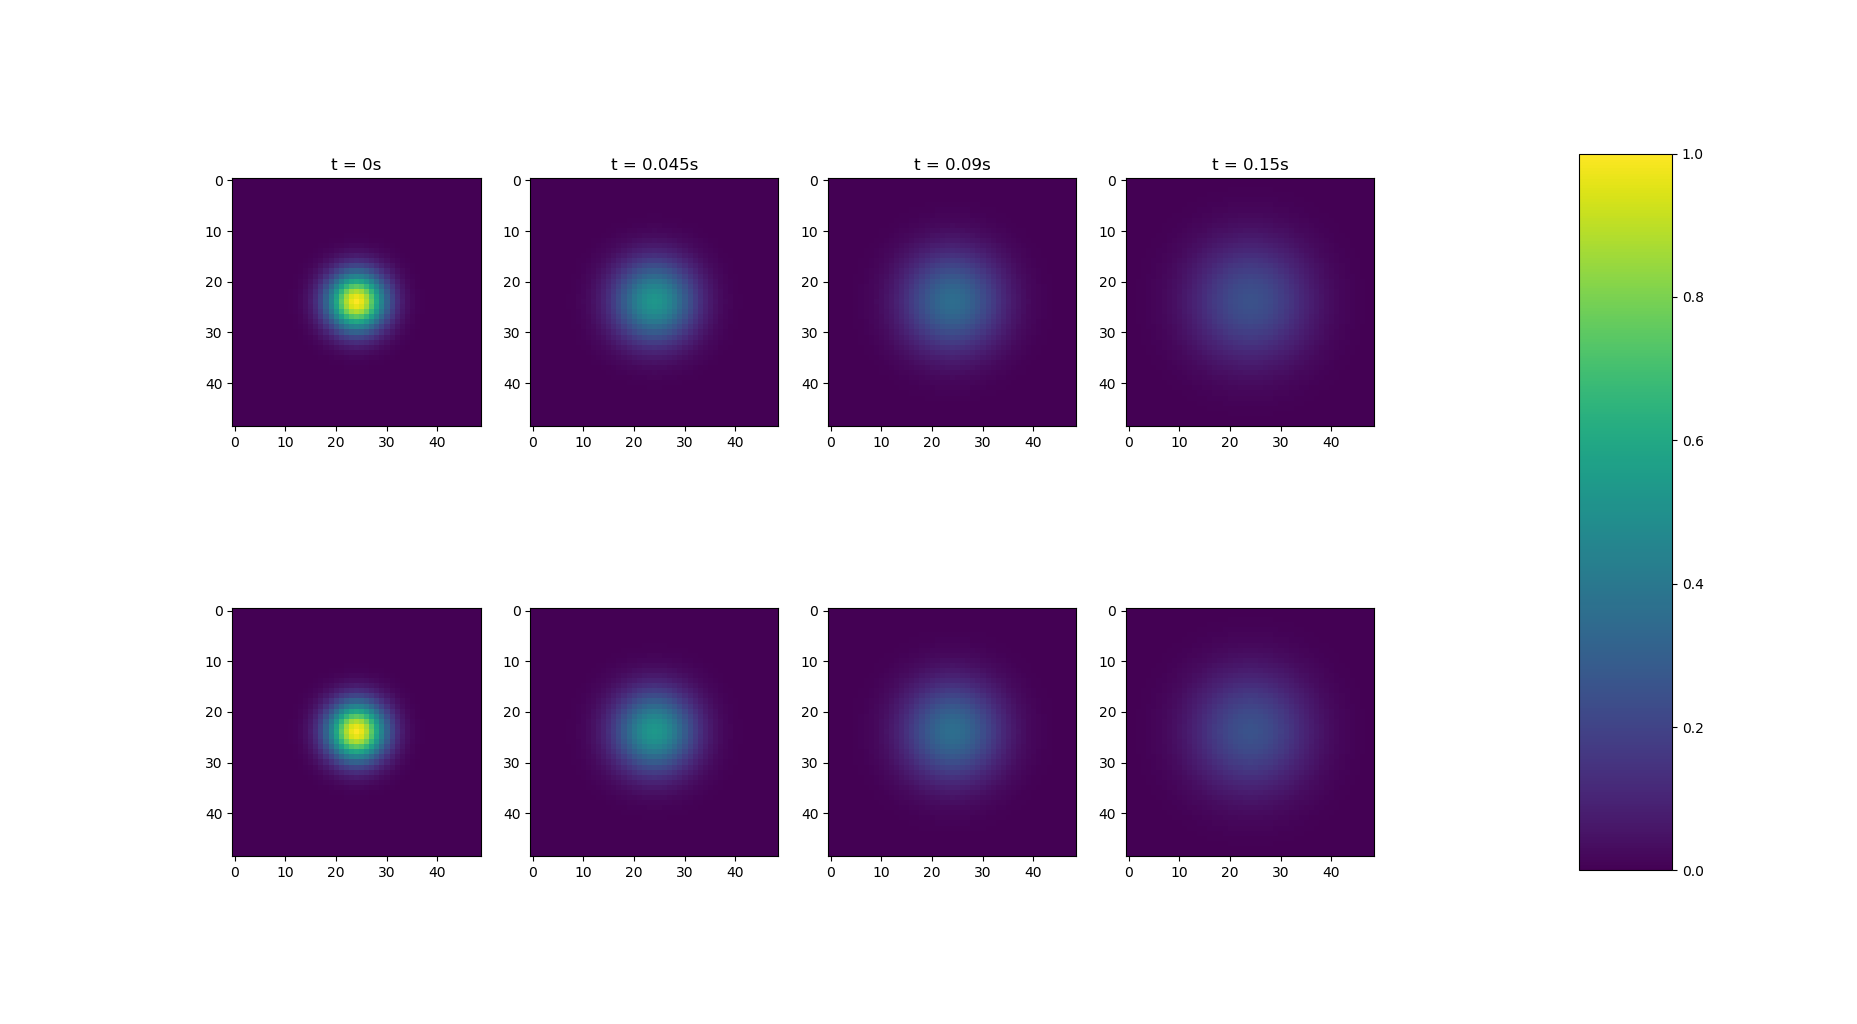
\includegraphics[width=.9\linewidth]{2stable.png}
		\subcaption{Stable solution for $\Delta t = 0.0015$, with all plots normalized to the same scale}
	\end{subfigure}
\caption{Comparison of a stable and unstable solution for the BVP}
\end{figure}
In order to use appropriate timesteps for FE, a stability limit for $\Delta t$ has to be derived.
The stability of a time stepping scheme can be analyzed by looking at the eigenvalues of the stepping scheme. For this $\lambda$ is considered to be an eigenvalue of the negative Laplacian and $\sigma$ is considered to be an eigenvalue of the time stepping scheme. 
\begin{equation}
	C = I - \Delta t A
\end{equation}
For some eigenvector $\mathbf{x}_m$ it holds that 
\begin{align}
C \mathbf{x}_m &= (I - \Delta t A)\mathbf{x}_m\\
C \mathbf{x}_m &= I\mathbf{x}_m - \Delta t A\mathbf{x}_m\\
\sigma_m \mathbf{x}_m &= \mathbf{x}_m - \Delta t \lambda_m \mathbf{x}_m\\
\sigma_m \mathbf{x}_m &= (1 - \Delta t \lambda_m )\mathbf{x}_m\\
\end{align}
Thus the relationship for the eigenvalues of the negative Laplacian ($\lambda$) and the eigenvalues of the time stepping scheme ($\sigma$) are related by $ \sigma_m = 1 - \Delta t \lambda_m$.
For FE to be stable $\left| \sigma_m\right|  \leq 1$ for all $\sigma_m$. Thus
\begin{align}
\lambda_{k_{x}, k_{y}}&=\frac{4}{h^{2}}\left[\sin ^{2}\left(\frac{\pi k_{x}}{2 N_{x}}\right)+\sin ^{2}\left(\frac{\pi k_{y}}{2 N_{y}}\right)\right]
\end{align}
Thus $lambda_m$ is bounded.
\begin{align}
0\leq\lambda_{m}&\leq\frac{4}{h^{2}}\\
\left| 1 - \Delta t \lambda_m \right| &\leq 1\\
\Delta t \lambda_m &\leq 2\\
\Delta t \frac{4}{h^{2}} &\leq 2\\
\Delta t  &\leq \frac{h^{2}}{2}
\end{align}

Calculating the stability limit for $h=0.08$ it can be seen that $\Delta t \leq 0.0016$. As previously only one time step was stable, which explains the blow-up of the solution for $\Delta t = 0.005 \text{ and } 0.003$.

By running the simulation for different values of h, with a stable time step for FE and a time step of 0.015 for BE, the speed of an implicit vs explicit method can be compared.

\begin{table}[H]
	\centering
\begin{tabular}{c|c|c}
	h 	 & FE & BE \\ \hline
	0.08 &0.163 s&0.107 s\\ \hline
	0.04 &0.968 s&0.650 s    \\ \hline
	0.02 &7.986 s&4.412 s    \\ \hline
\end{tabular}
\caption{Time to solve the BVP for different step-sizes with FE and BE}
\end{table}

It can be seen that solving the system implicitly is always faster for this range of h than the explicit solution, as the required time step decreases rapidly such that solving a linear system is less computational effort than performing more steps.

\section{Time evolution of the wave equation}
In order to examine the time evolution of the wave equation, the following BVP is considered.
\begin{equation}
\begin{aligned} \frac{\partial^{2} u}{\partial t^{2}} &=c^{2} \Delta u+f, \quad(x, y) \in(0,4) \times(0,12), \quad t \in[0,8] \\ u(x, y, t) &=0, \quad(x, y) \in \partial \Omega, \quad t \in[0,8] \\ u(x, y, 0) &=0, \quad(x, y) \in \Omega \\\left.\frac{\partial u}{\partial t}\right|_{t=0} &=0, \quad(x, y) \in \Omega \\ f(x, y, t) &=\sin (2 \pi \nu t) e^{\alpha(x-2)^{2}+\alpha(y-2)^{2}} \quad(x, y) \in \overline{\Omega}, \quad t \in[0,8] \\ \quad \text { with } \alpha=-50, & \nu=4 \end{aligned}
\end{equation}
With $\overline{\Omega} = \left[0,4\right]\times \left[0,12\right]$. 
The discretization of the Laplacian Operator is performed using a central finite difference method on a doubly uniform grid with step h.
\begin{equation}
L=\frac{1}{h^2}
\begin{bmatrix}
-2&1&0&\dots&0\\
1&-2&1& &\vdots\\
0&1&-2&1&\\
\vdots&&&\ddots&\\
0&\dots&0&1&-2
\end{bmatrix}
\label{eq:Laplacian}
\end{equation}
From this the space discrete form can be determined to be
\begin{equation}
\frac{\partial^2 \mathbf{u}}{\partial t^2} \approx c^2 L \mathbf{u} + f
\end{equation}
In order to use time stepping on the second derivative in time, a finite difference time discretization (FDTD) is used.
\begin{align}
\frac{\partial^2 \mathbf{u}^k}{\partial t^2} &= \frac{\mathbf{u}^{k-1}-2\mathbf{u}^{k}+\mathbf{u}^{k+1}}{\Delta t ^2}+\mathcal{O}(\Delta t^2)\\
 c^2 L \mathbf{u}^k +f &\approx \frac{\mathbf{u}^{k-1}-2\mathbf{u}^{k}+\mathbf{u}^{k+1}}{\Delta t ^2}\\
\mathbf{u}^{k+1} &\approx c^2 \Delta t ^2 L \mathbf{u}^k +\Delta t ^2 f + 2\mathbf{u}^{k} - \mathbf{u}^{k-1}\\
\mathbf{u}^{k+1} &\approx (c^2 \Delta t ^2 L+ 2I)\mathbf{u}^{k} - \mathbf{u}^{k-1} +\Delta t ^2 f
\end{align}
In order to approximate the initial conditions with sufficient accuracy, $\mathbf{u}^{1}$ is expanded as a Taylor series around $\mathbf{u}^{0}$.
\begin{equation}
\mathbf{u}^{1}=\mathbf{u}^{0}+\Delta t \frac{\partial \mathbf{u}^{0}}{\partial t} + \frac{\Delta t^2}{2} \frac{\partial^2 \mathbf{u}^{0}}{\partial t^2} + \mathcal{O}(\Delta t^3)
\end{equation}
As it is given that $\frac{\partial \mathbf{u}^{0}}{\partial t} = 0$ and that $\frac{\partial^2 \mathbf{u}^{0}}{\partial t^2} \approx c^2 L \mathbf{u}^0 + f$ The first step can be calculated as.
\begin{equation}
\mathbf{u}^{1}=\mathbf{u}^{0}+ \frac{\Delta t^2 c^2}{2} L \mathbf{u}^{0} + \frac{\Delta t^2 }{2} f+ \mathcal{O}(\Delta t^3) 
\end{equation}
In order to guarantee a stable time stepping, the simulation is run at 99\% of the corresponding Courant–Friedrichs–Lewy (CFL) number. This number is a important dimensionless number, which relates the speed of the wave to the corresponding spatial and time steps used.
\begin{equation}
C = \frac{c\Delta t}{\sqrt{2}h}
\end{equation}
Running the simulation for $c=1$ on a grid with $h=0.02$ yields the follwing solution.

\begin{figure}[H]
	\centering
	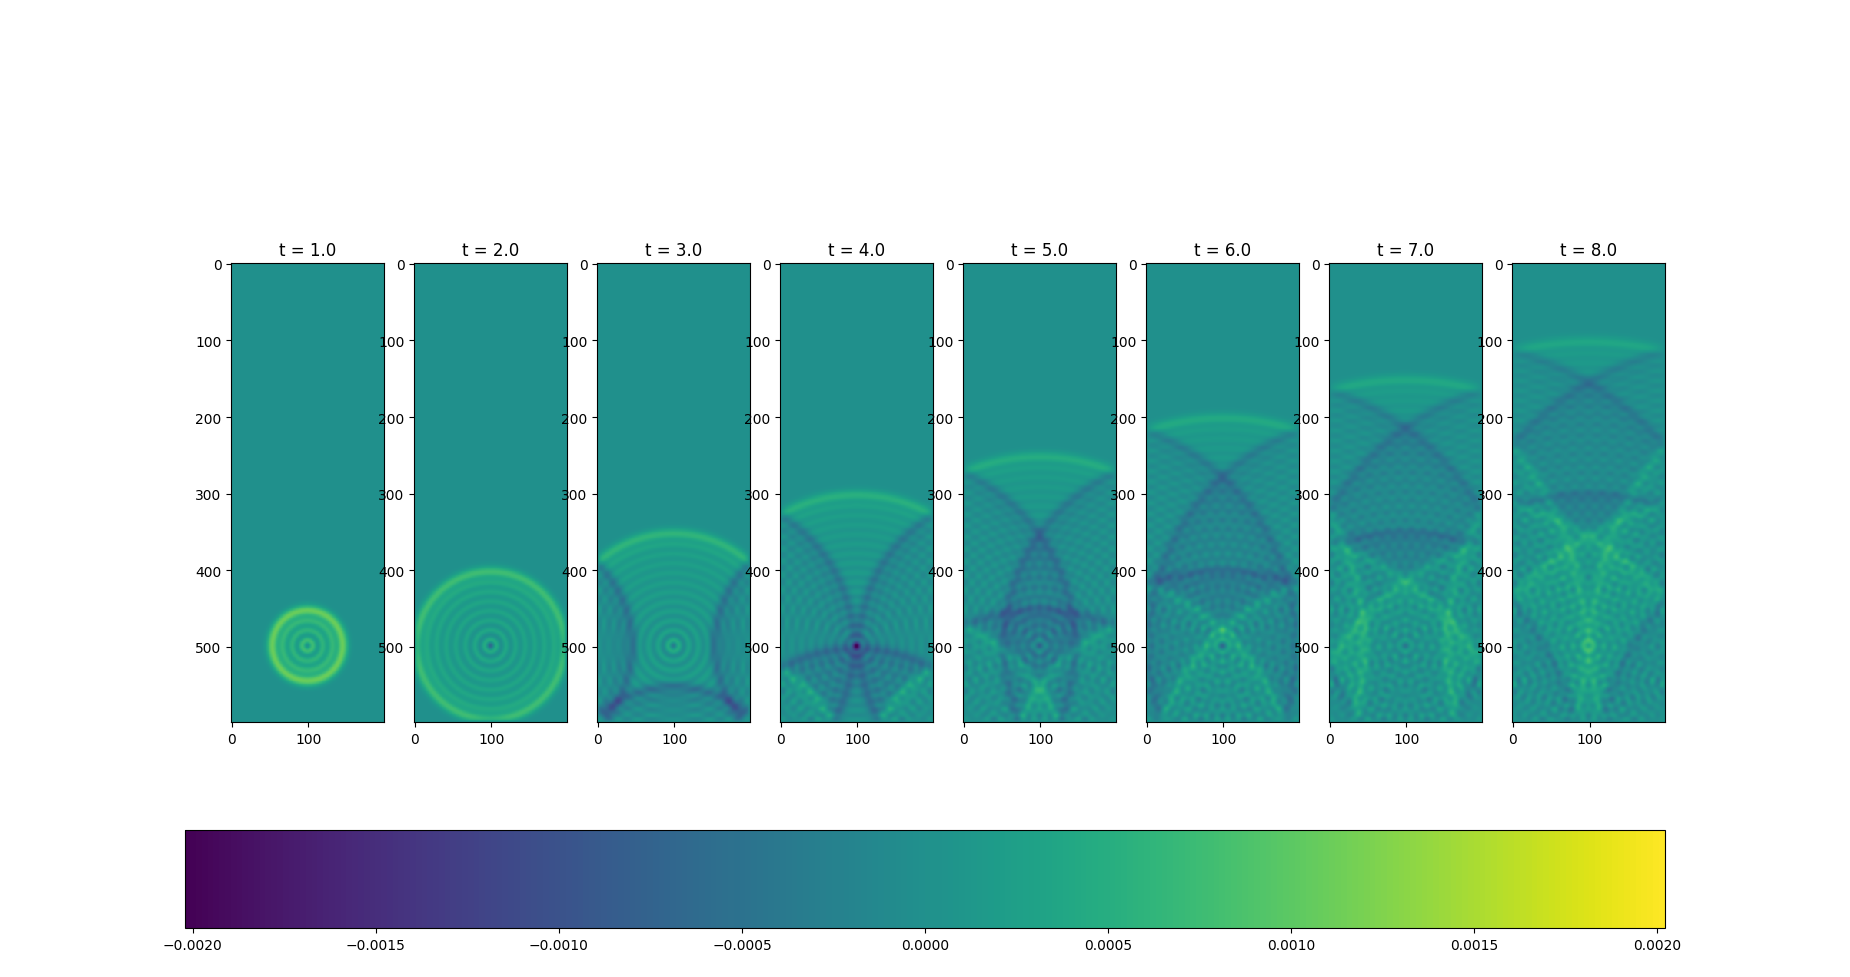
\includegraphics[width=.9\linewidth]{311.png}
	\caption{Solution of the wave equation on a uniform grid with step 0.02 and a wavespeed of 1}
	\label{fig:c1}
\end{figure}
It can clearly be seen that the wavefront travels at a speed of 1 unit per secodn, which is expected as $c=1$. Furthermore, reflection can be observed at the boundaries, which however flip the orientation of the wave, whcich would not be expected in a physical system. This behaviour comes from the use of homogeneous dirichlet conditions on the boundary of the domain. When performing a similar the simulation with $c=2$ it can be seen that the wave travels twice as fast.

\begin{figure}[H]
	\centering
	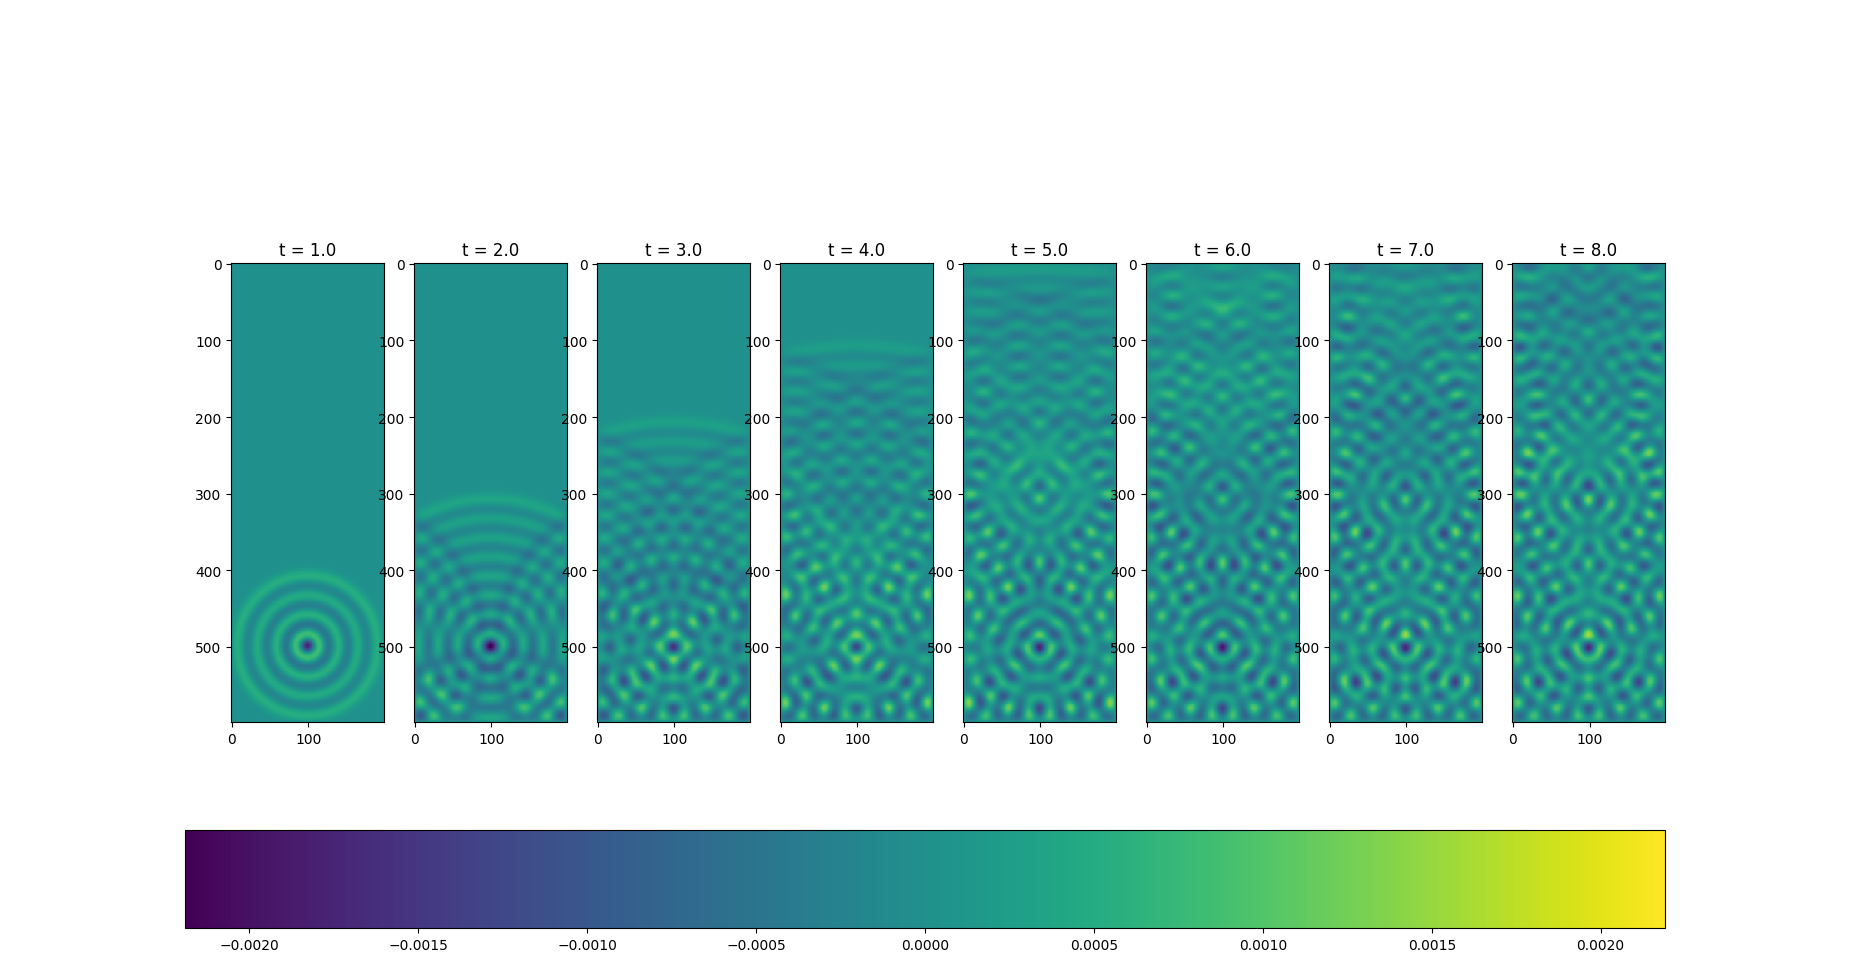
\includegraphics[width=.9\linewidth]{31.png}
	\caption{Solution of the wave equation on a uniform grid with step 0.02 and a wavespeed of 2}
	\label{fig:c2}
\end{figure}
In contrast to the previous simulation, standing waves can be observed. Furthermore shifted replicas of the source are present in later solutions. Changing the speed of the wave slightly destroys these inferences. it can therefore be assumed that these patterns come from standing waves developing between the boundaries. This can be expected as the frequency of the source function permits an integer number of wavelengths to travel to each boundary. This however is also the case for $c=1$ and no such pattern is visible at 8 seconds. Thus both simulations are run for 300 and 600 seconds to reach a quasi steady state and the results are compared. The simulation for $c=1$ is run twice as long, to allow the waves to travel the same distance as for $c=2$.
\begin{figure}[H]
	\begin{subfigure}{.5\textwidth}
		\centering
		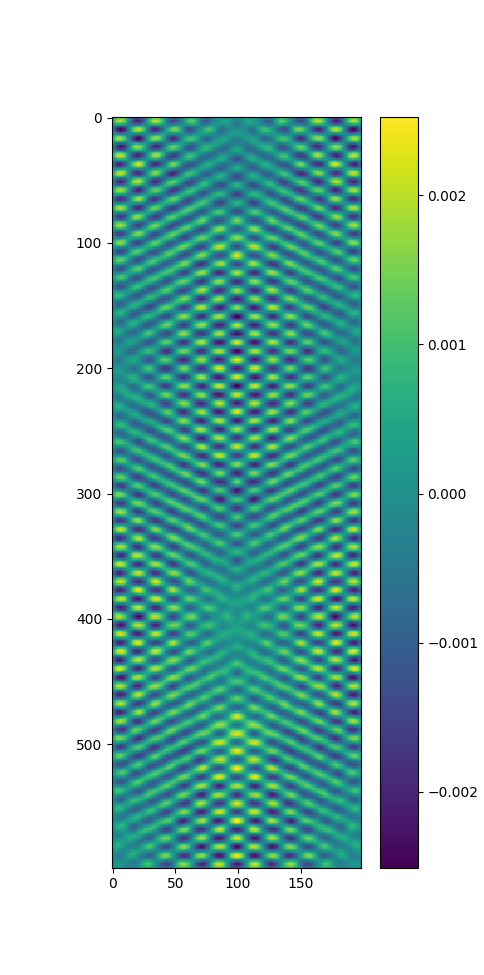
\includegraphics[width=.9\linewidth]{3steadyc=1.png}
		\subcaption{Quasi-steady solution for c=1 at t=600s}
	\end{subfigure}
	\begin{subfigure}{.5\textwidth}
		\centering
		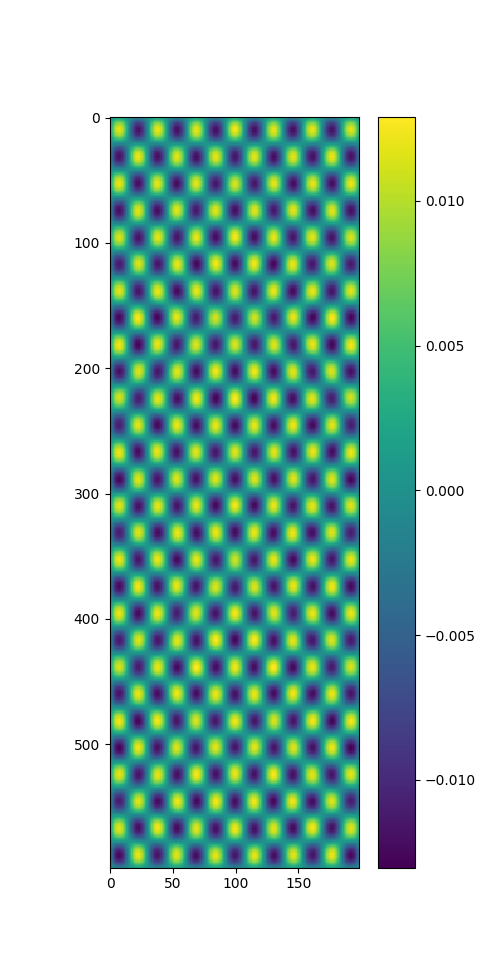
\includegraphics[width=.9\linewidth]{3steadyc=2.png}
		\subcaption{Quasi-steady solution for c=2 at t=300s}
	\end{subfigure}
	\caption{Comparison of the quasi-steady solutions}
\end{figure}
From these 2 figures it can be seen that the patterns emerging in \autopageref{fig:c1} and \autopageref{fig:c2}, are indeed standing waves.

\section{Numerical Solutions of the Fisher equation}
This section discusses numerical solutions of the unsteady fisher equation on a 2-dimensional, for this the following BVP with initial conditions is considered.
\begin{equation}
\begin{aligned} \frac{\partial u}{\partial t} &=\Delta u+k u(1-u), \quad(x, y) \in(0,16) \times(0,8), \quad t \in(0,40] \\ u(x, y, t) &=0, \quad(x, y) \in \partial \Omega, \quad t \in(0,40] \\ u(x, y, 0) &=e^{-2(x-1.5)^{2}-2(y-1.5)^{2}} \quad(x, y) \in \overline{\Omega} \\ k(x, y) &=\left\{\begin{array}{ll}{\alpha,} & {(x, y) \in \Omega_{1}} \\ {0,} & {\text { otherwise }}\end{array}\right.\end{aligned}
\end{equation}
With $\alpha = 1$, $\overline{\Omega} = \left[0,16\right]\times\left[0,8\right]$ and $\Omega_1 = \bigcup\limits_{i=1}^{5} R_{i}$.
\begin{equation}
\begin{array}{l}{R_{1}=[1,2] \times[1,2]} \\ {R_{2}=[1,3] \times[3,5]} \\ {R_{3}=[4,7] \times[4,7]} \\ {R_{4}=[9,12] \times[4,6]} \\ {R_{5}=[13,15] \times[1,3]}\end{array}
\end{equation}
For the spatial discretisation, a FDM Method is used, in which the Laplacian can be discretized as $L$, \autoref{eq:Laplacian}. With this, the discrete equation becomes, where $\mathbf{k}$ is the lexicographic vector of coefficients k, and $\circ$ denotes the hadamard product of 2 vectors.
\begin{equation}
\frac{\partial \mathbf{u}}{\partial t} = L \mathbf{u} + \mathbf{k}\circ\mathbf{u}\circ(1-\mathbf{u})
\end{equation}

In order to solve this semi discrete problem, a time stepping scheme has to be employed. As an explicit scheme, Forward Euler can be used. With this scheme, the fully discrete equation becomes
\begin{equation}
\mathbf{u}^{n+1} = \mathbf{u}^n+\Delta t*\left(L \mathbf{u}^n + \mathbf{k}\circ\mathbf{u}^n\circ\left(1-\mathbf{u}^n\right)\right)
\end{equation}
In order to achieve a stable solution, $\Delta t$ is set to be at 99\% of the stability margin for the linear part of the equation. $\Delta t = 0.99*\frac{h^2}{4}$. With this the solution on the domain can be computed for different grid spacings.
\begin{figure}[H]
	\centering
	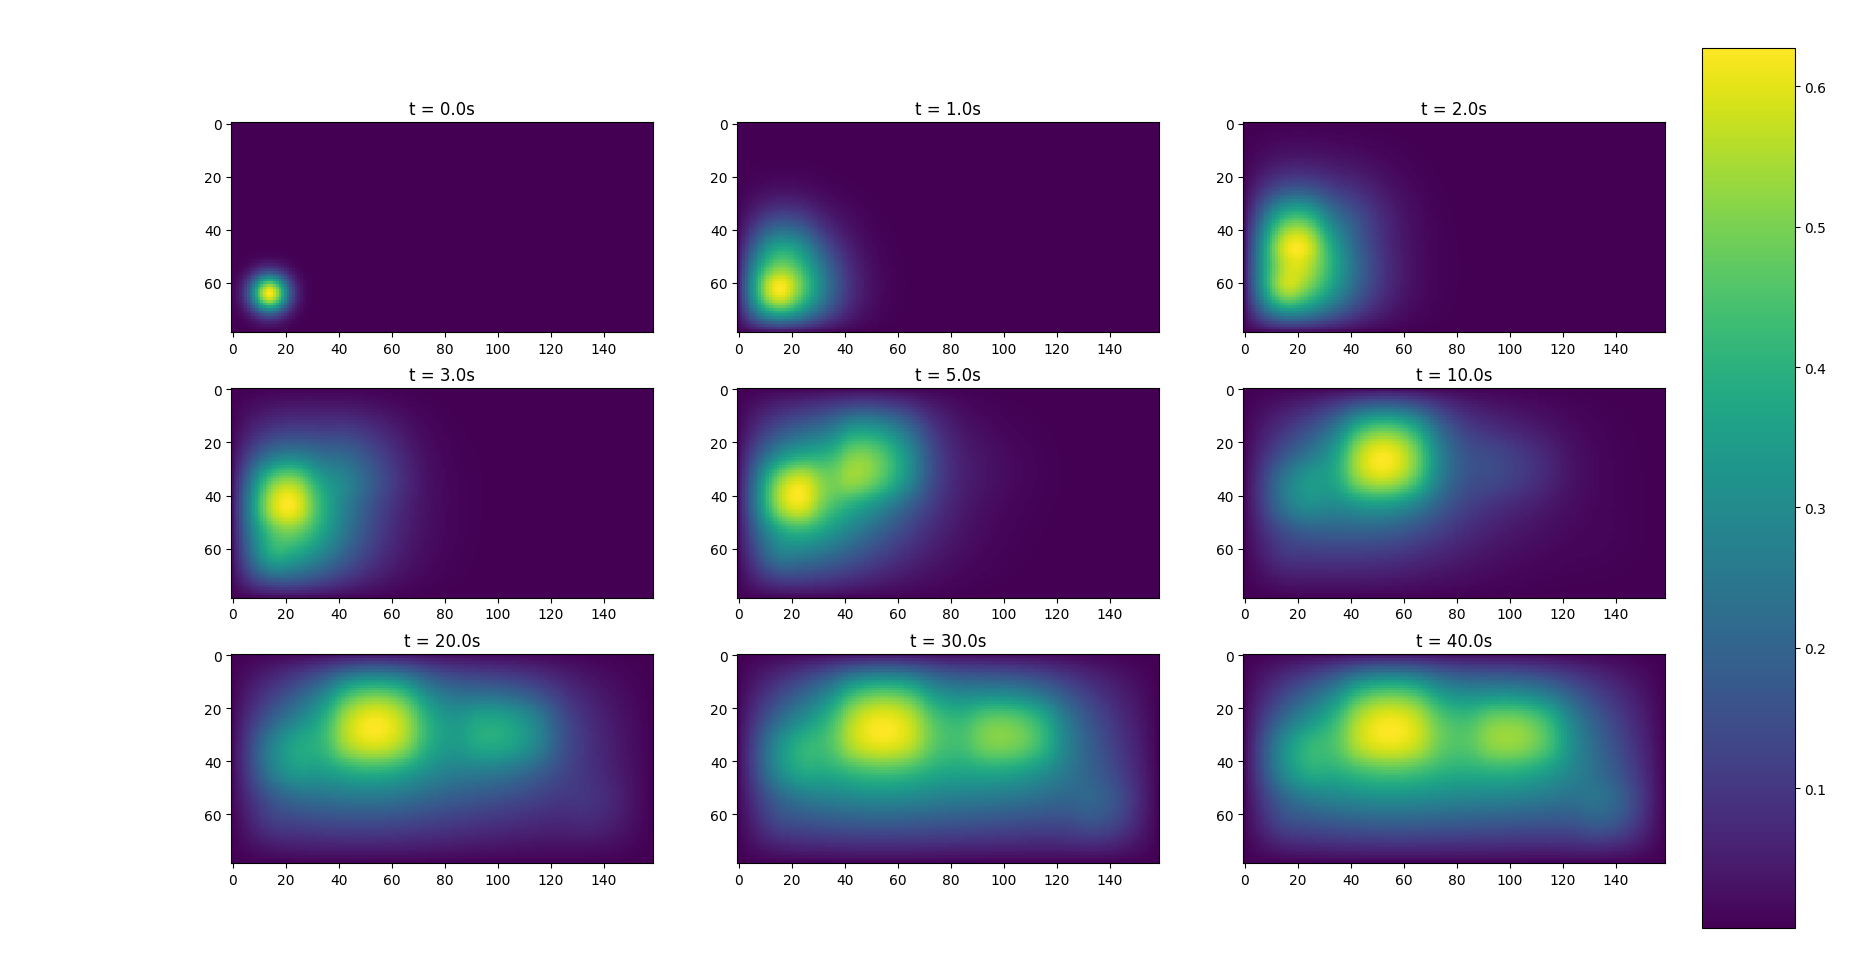
\includegraphics[width=.9\linewidth]{4FE.png}
	\caption{Solution of the Fisher equation on a grid with $h=0.04$, with FE time stepping}
\end{figure}
As an implicit time stepping scheme, backwards Euler is used.
\begin{align}
\mathbf{u}^{n+1} = \mathbf{u}^n+\Delta t*f(\mathbf{u}^{n+1})\\
f(\mathbf{u}^{n+1})=L \mathbf{u}^{n+1} + \mathbf{k}\circ\mathbf{u}^{n+1}\circ\left(1-\mathbf{u}^{n+1}\right)
\end{align}
As this equation is neither explicit nor linear, a non-linear solver has to be implemented. For this Newton-Raphson is chosen. At every inner iteration i of this method, the solution is updated to.
\begin{equation}
\mathbf{u}_{i+1}^{n+1}=\mathbf{u}_{i}^{n+1}-\left[I-\Delta t J\left(\mathbf{u}_{i}^{n+1}\right)\right]^{-1}\left[\mathbf{u}_{i}^{n+1}-\mathbf{u}^{n}-\Delta t \mathbf{f}\left(\mathbf{u}_{i}^{n+1}\right)\right]
\end{equation}
The jacobian at every iteration is calculated as
\begin{equation}
J\left(\mathbf{u}_{i}^{n+1}\right)=L+\operatorname{diag}(\mathbf{k})-2 \operatorname{diag}(\mathbf{k})\operatorname{diag}(\mathbf{u}_{i}^{n+1})
\end{equation}
in which $\operatorname{diag}(\mathbf{x})$ is the diagonal matrix with $\mathbf{x}$ on its diagonal. The update at each inner iteration $\mathbf{v}_i = \left[I-\Delta t J\left(\mathbf{u}_{i}^{n+1}\right)\right]^{-1}\left[\mathbf{u}_{i}^{n+1}-\mathbf{u}^{n}-\Delta t \mathbf{f}\left(\mathbf{u}_{i}^{n+1}\right)\right]$, includes the inverse of a matrix, which is computationally very expensive to solve, thus the following sparse linear system is solved instead.
\begin{equation}
\left[I-\Delta t J\left(\mathbf{u}_{i}^{n+1}\right)\right] \mathbf{v}_i = \left[\mathbf{u}_{i}^{n+1}-\mathbf{u}^{n}-\Delta t \mathbf{f}\left(\mathbf{u}_{i}^{n+1}\right)\right]
\end{equation}
And the solution is updated to
\begin{equation}
	\mathbf{u}^{n+1}_{i+1} = 	\mathbf{u}^{n+1}_{i} - \mathbf{v}_i
\end{equation}
The inner iterations are stopped when $\norm{\mathbf{v}_i} < \epsilon$.
For this problem $\epsilon$ was set to be $10^-3$, and $\Delta t = 0.4$, was found to solve the equation the fastest. From the convergence plot, the quadratic convergence of Newton-Raphson can clearly be identified on the residuals. Furthermore it can be seen that all outer iterations take at least 2, but at most 4 inner iterations to converge. This fast convergence in connection with the big time steps that can be used, can make it a viable alternative to FE.
\begin{figure}[H]
	\centering
	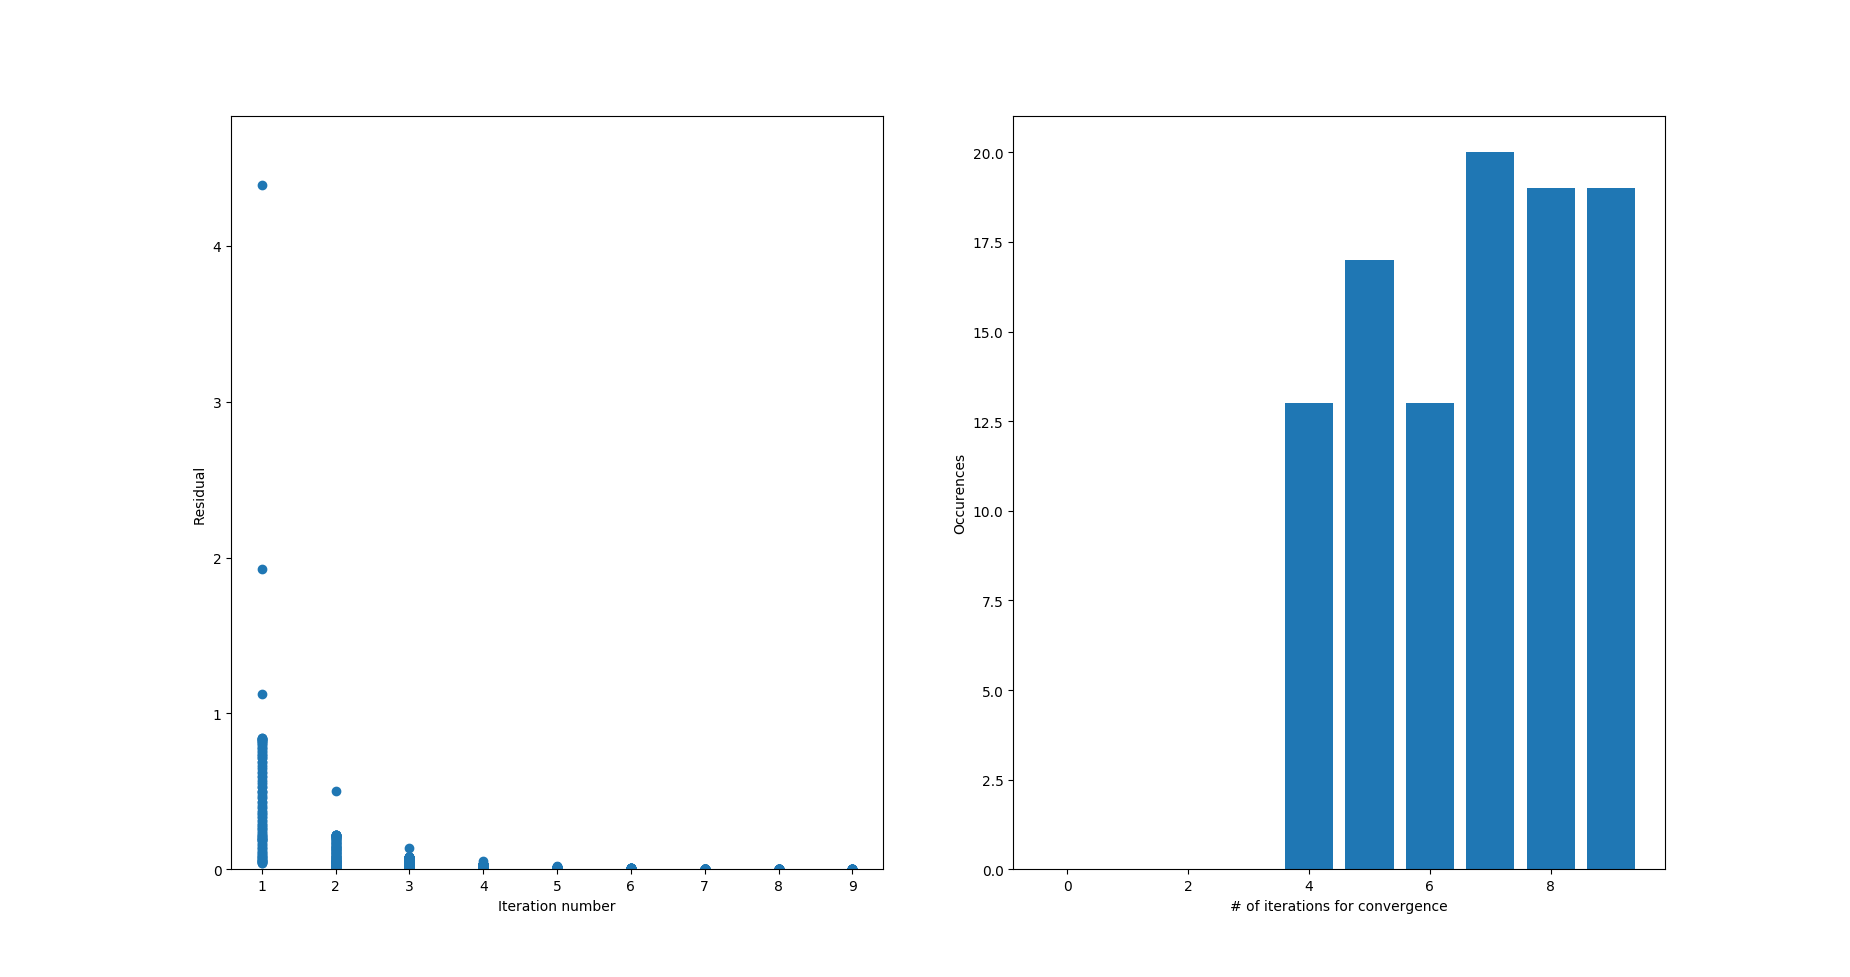
\includegraphics[width=.9\linewidth]{4ConvergenceNewton.png}
	\caption{Convergence history of BE-NR method.}
\end{figure}

Both implicit and explicit computation times were recorded for different grid spacings with both methods.
\begin{table}[H]
\centering
\begin{tabular}{c|c|c}
	h & FE & BE-NR \\\hline
	0.1 & 5s & 5s\\ \hline
	0.08 & 11s & 18s\\ \hline
	0.04 & 198s & 130s
\end{tabular}
\caption{Comparison of computing times for different grid spacings and time stepping schemes. Run on an Intel Core i5-3570 CPU  4 Cores @ 3.40GHz}
\end{table}
It can be seen that Backwards Euler takes approximately the same time for big h, however as h decreases BE-NR becomes faster. This most likely originates from the fact that the computational cost of the linear solves grows slower than the increase of needed time steps for FE.\par
As a secondary nonlinear solver for BE a Picard method is investigated, in which the update in the inner iterations is calculated with
\begin{align}
\mathbf{u}_{i+1}^{n+1}=\Delta t \mathbf{f}^{n+1}\left(\mathbf{u}_{i}^{n+1}\right)+\mathbf{u}^{n}\\
f(\mathbf{u}^{n+1})=L \mathbf{u}^{n+1} + \mathbf{k}\circ\mathbf{u}^{n+1}\circ\left(1-\mathbf{u}^{n+1}\right)
\end{align}
The inner iterations of Picards method are stopped when $\norm{\mathbf{u}_{i}^{n+1}-\Delta t \mathbf{f}^{n+1}\left(\mathbf{u}_{i}^{n+1}\right)-\mathbf{u}^{n}} < \epsilon$, which is chosen to be $10^{-3}$. As a first guess for $\Delta t$, the same step as for FE is used. However this time step, makes the solver unstable and the solution explodes rapidly. Thus $\Delta t$ is halved, which leads to a stable solution. By analyzing the convergence plot, it can be seen that convergence is very fast and most outer iterations converge in 1 or 2 iterations, however $\Delta t$ is twice as small as for FE, which always takes only one step. Furthermore BE-Picard requires significantly more matrix multiplications than FE, and as such takes about 4 times as long to compute. From these results, it can be concluded that BE-Picard should not be used to solve this equation.

\begin{figure}[H]
	\centering
	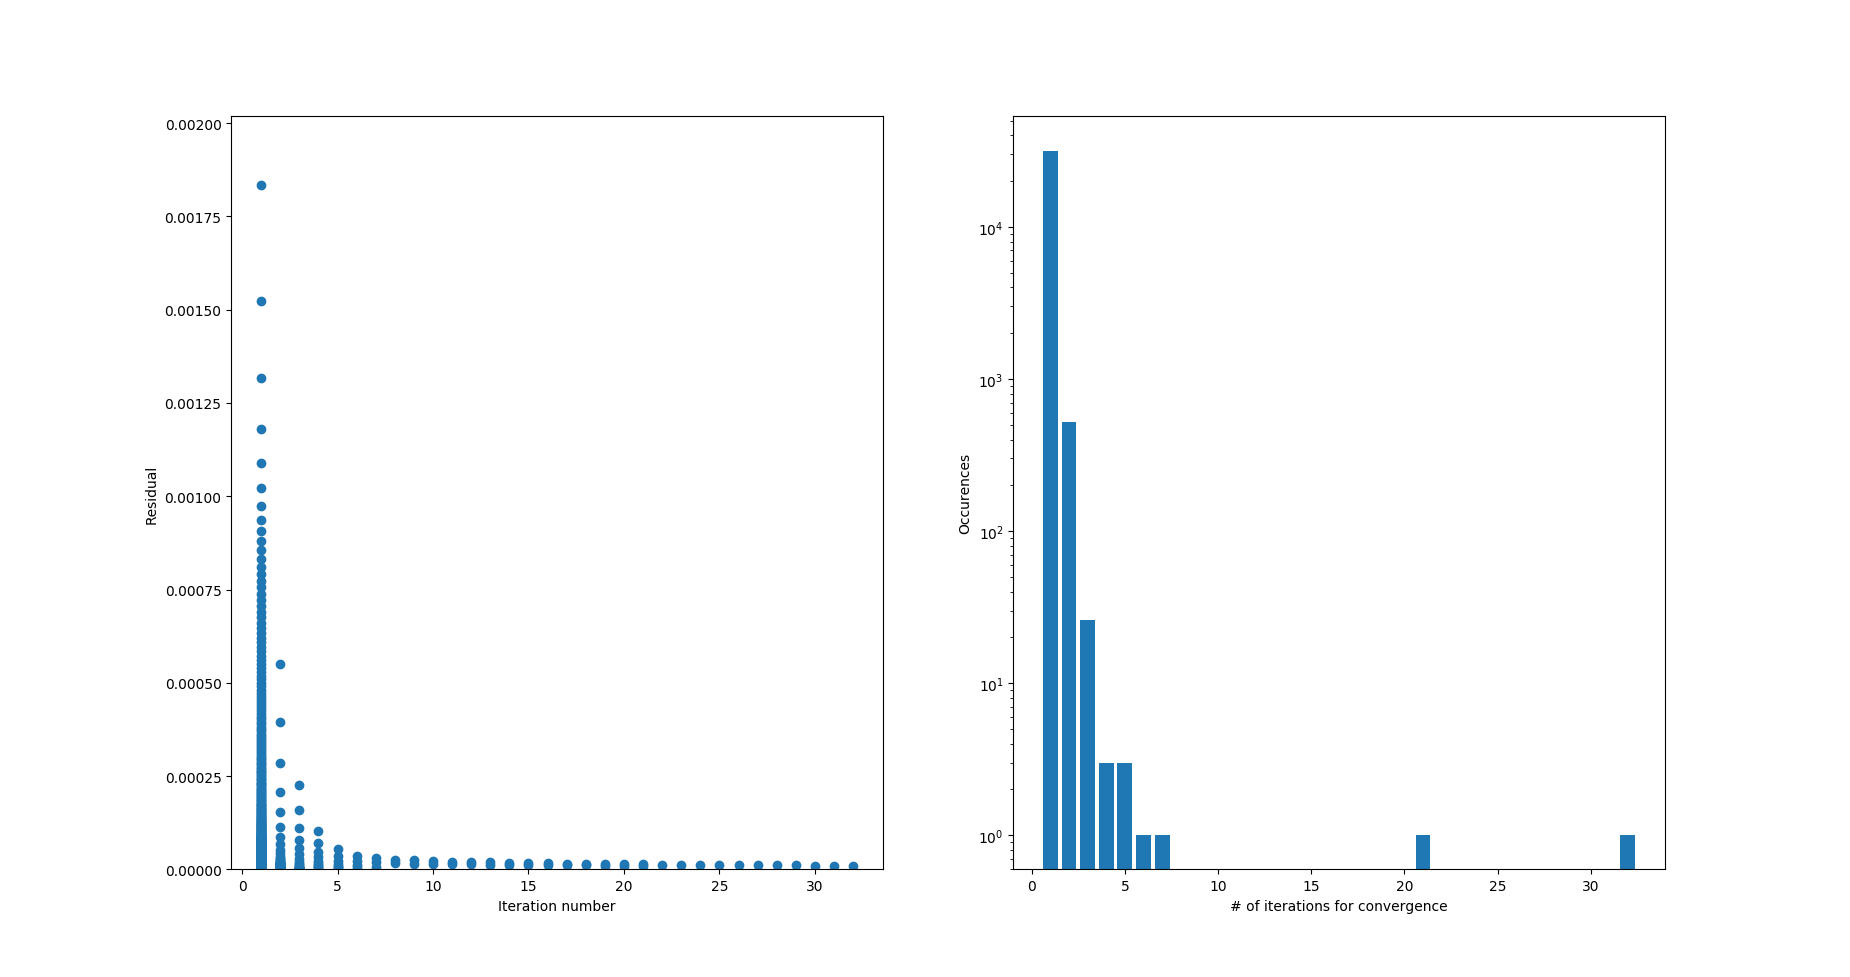
\includegraphics[width=.9\linewidth]{4ConvergencePicard.png}
	\caption{Convergence history of BE-Picard method.}
\end{figure}

In order to explore the solution dynamics of the Fisher equation $\alpha$ is set to 10. It can be seen that the solution accumulates on $\Omega_1$ a lot faster and the edges of the accumulation are sharper. Furthermore, smaller regions like $\left[1,2\right]\times\left[1,2\right]$ experience a higher accumulation, than with a smaller $\alpha$. When observing the later time evolution, it is apparent that a quasi steady state is reached faster with a higher $\alpha$.
\begin{figure}[H]
	\centering
	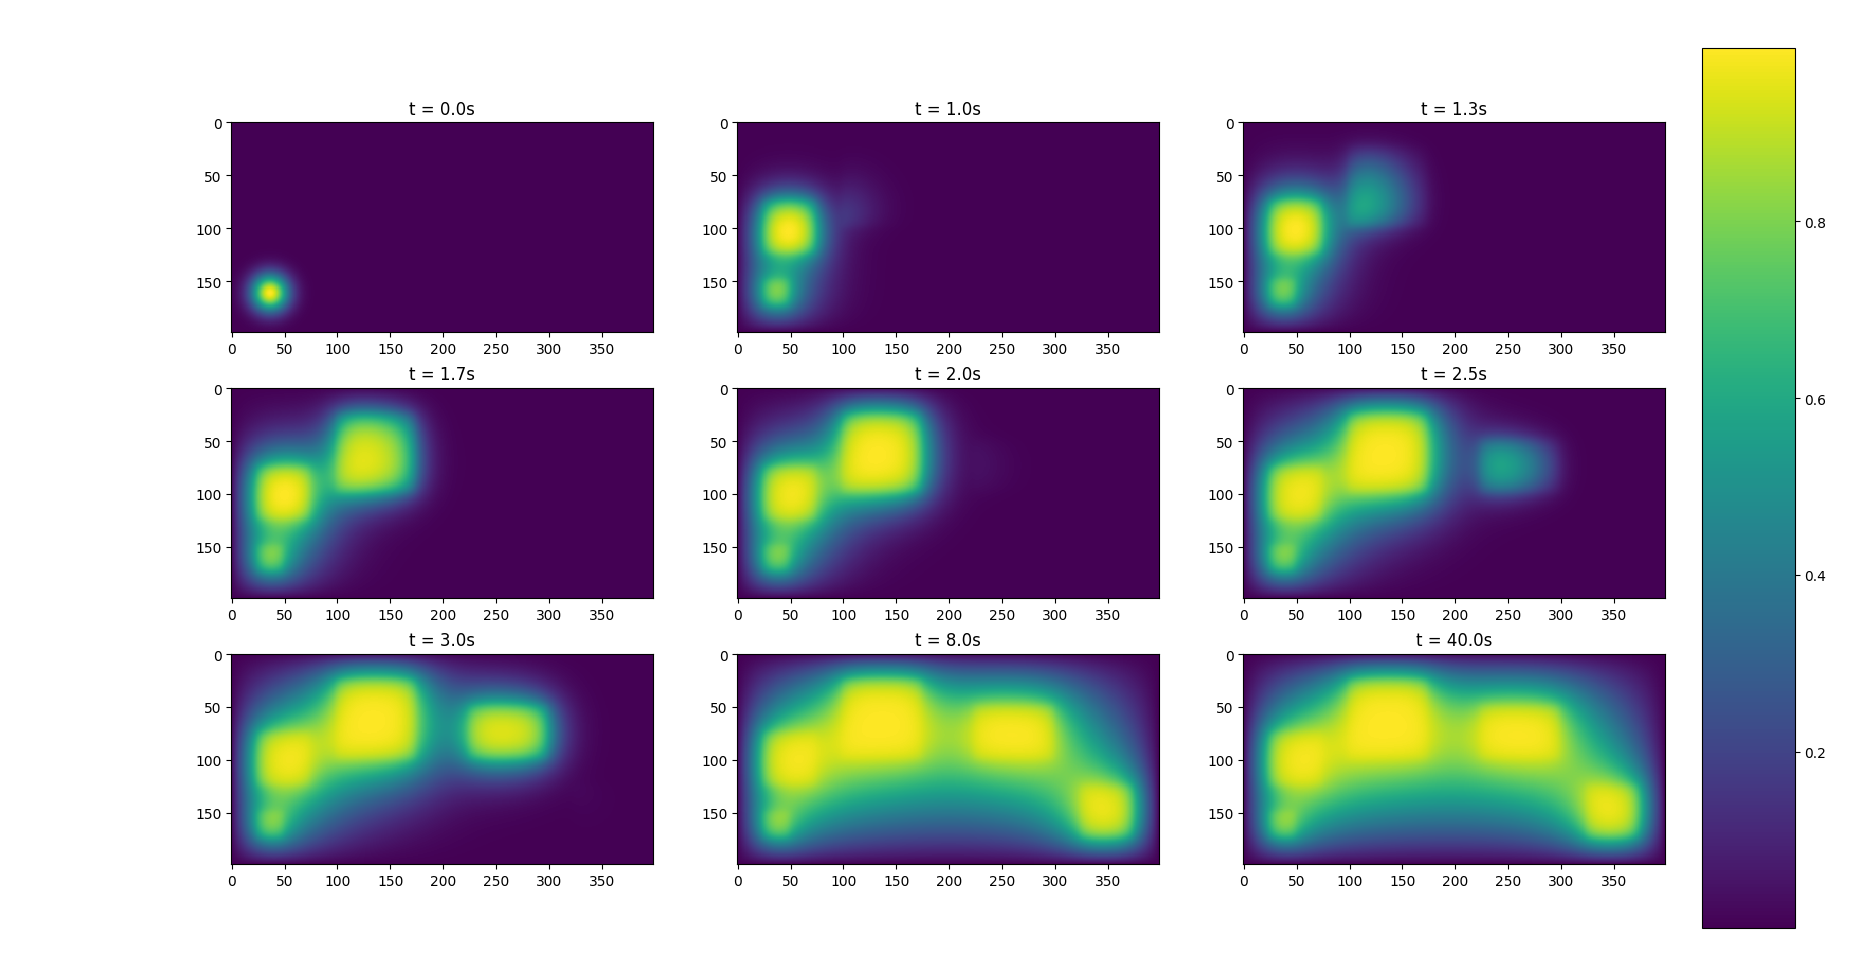
\includegraphics[width=.9\linewidth]{4solutiondynamics.png}
	\caption{Solution of the Fisher equation for $\alpha=10$ and $h=0.04$}
\end{figure}

\section{Convergence of GMRES}
The spsolve used in all problems until now is classified as a direct solver, which means that the solution of the system is calculated exactly in a single step, for which the most commonly a LU-Decomposition or an Incomplete-LU is used. Another class of linear solvers are iterative ones, an example for such a solver is the Generalized minimal residual method, which hinges on the subject of expressing the solution inside a Krylov subspace $\mathcal{K}_{r}(A, b)$ of $\mathbb{R}^n$.
In order to investigate the convergence of the GMRES algorithm, the following BVP is considered.
\begin{equation}
\begin{aligned}-\Delta u-\gamma u &=f, \quad(x, y) \in \Omega=(0,10) \times(0,10) \\ u(x, y) &=0, \quad(x, y) \in \partial \Omega \\ f(x, y) &=e^{-10(x-5)^{2}-10(y-5)^{2}} \quad(x, y) \in \Omega \end{aligned}
\end{equation}
This BVP is discretized using FDM on a doubly uniform grid. A such the equation in its discrete form can be written as
\begin{equation}
\left(L-\gamma I \right)\mathbf{u} = \mathbf{f}
\end{equation}
in which L is the discretization of the negative Laplacian and I is the Identity matrix of appropriate size.
With this, the BVP can be solved for $\gamma=-40,0 \text{ and } 40$, with spsolve and GMRES. For GMRES, the maximum number of iterations is set to 5000, furthermore restarting is disabled and the tolerance for convergence is set to $10^{-12}$.
\begin{figure}[H]
	\centering
	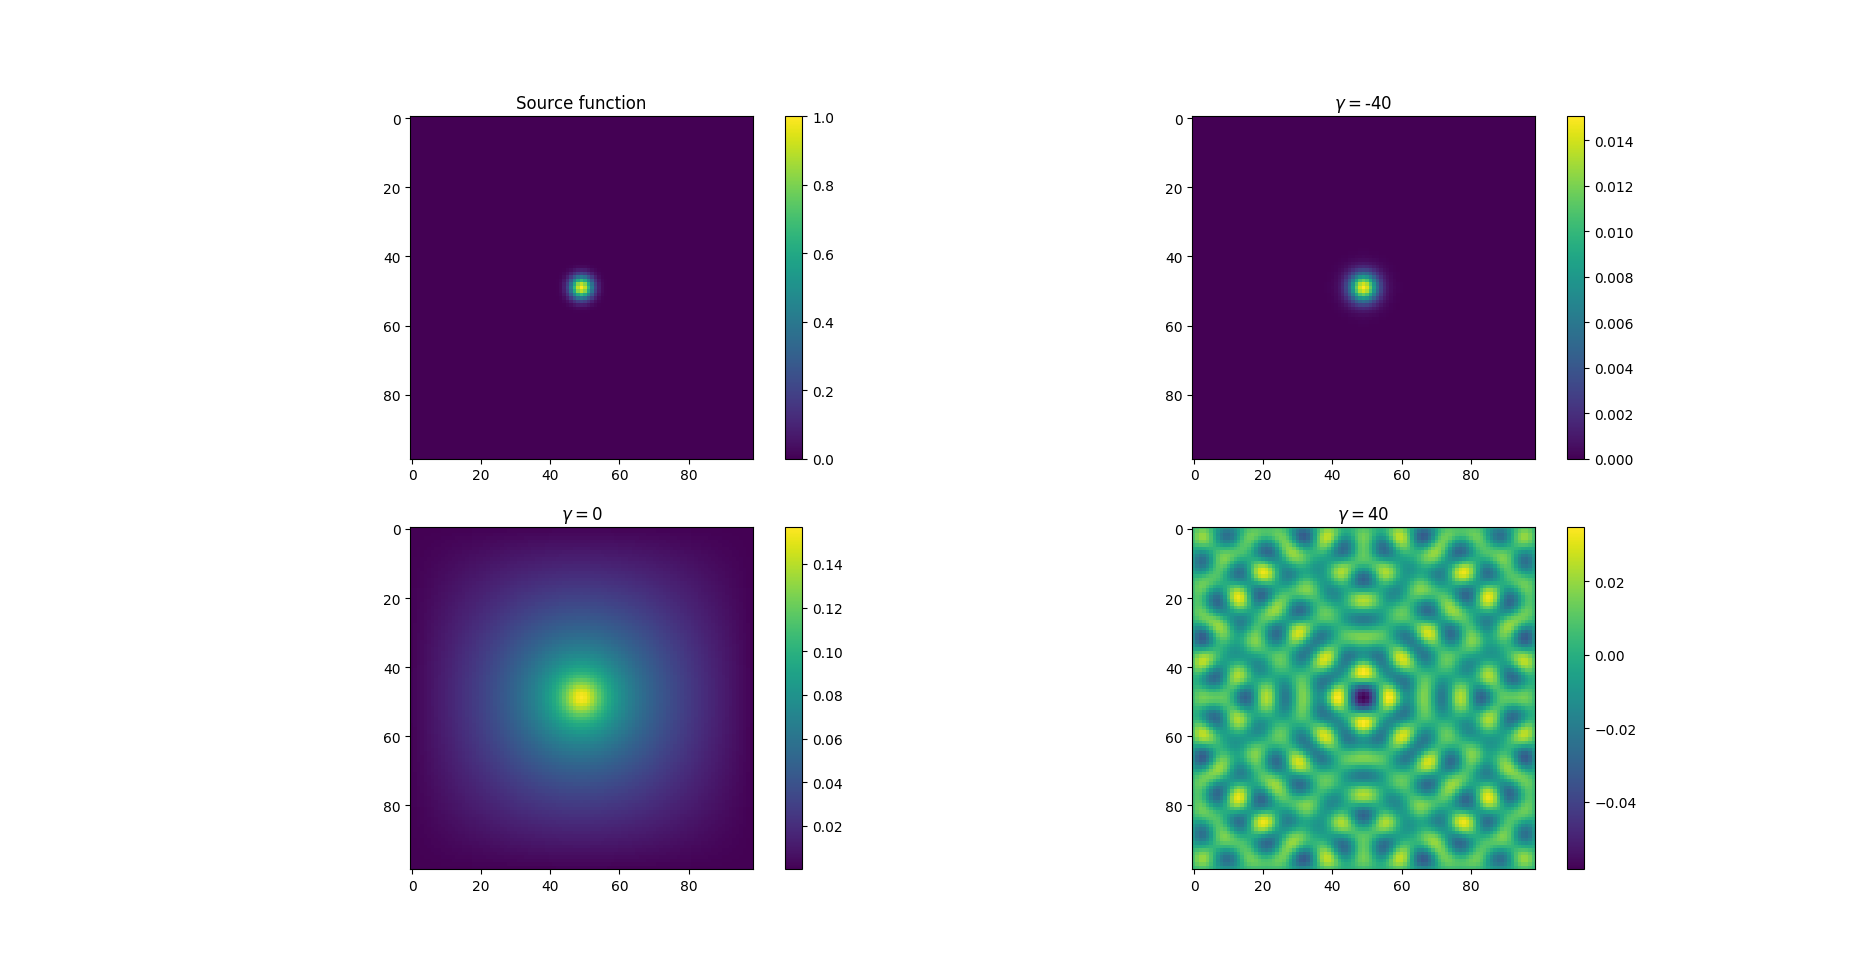
\includegraphics[width=.9\linewidth]{5sol.png}
	\caption{Solution of the BVP on the domain for $h=0.1$, solved by GMRES}
\end{figure}
When analyzing the convergence history of GMRES for different $\gamma$ it can be seen that convergence for $\gamma=-40$ is very fast, while for the other ones, the residual nearly stagnates for the first few iterations. However after an initial stagnation for $\gamma=0$, it converges with the approximately same rate as the convergence of $\gamma=-40$. In contrast to that the convergence for $\gamma=40$ plateaus frequently during the convergence after iteration 450, while the rate of convergence is considerably lower than the other two's.
\begin{figure}[H]
	\centering
	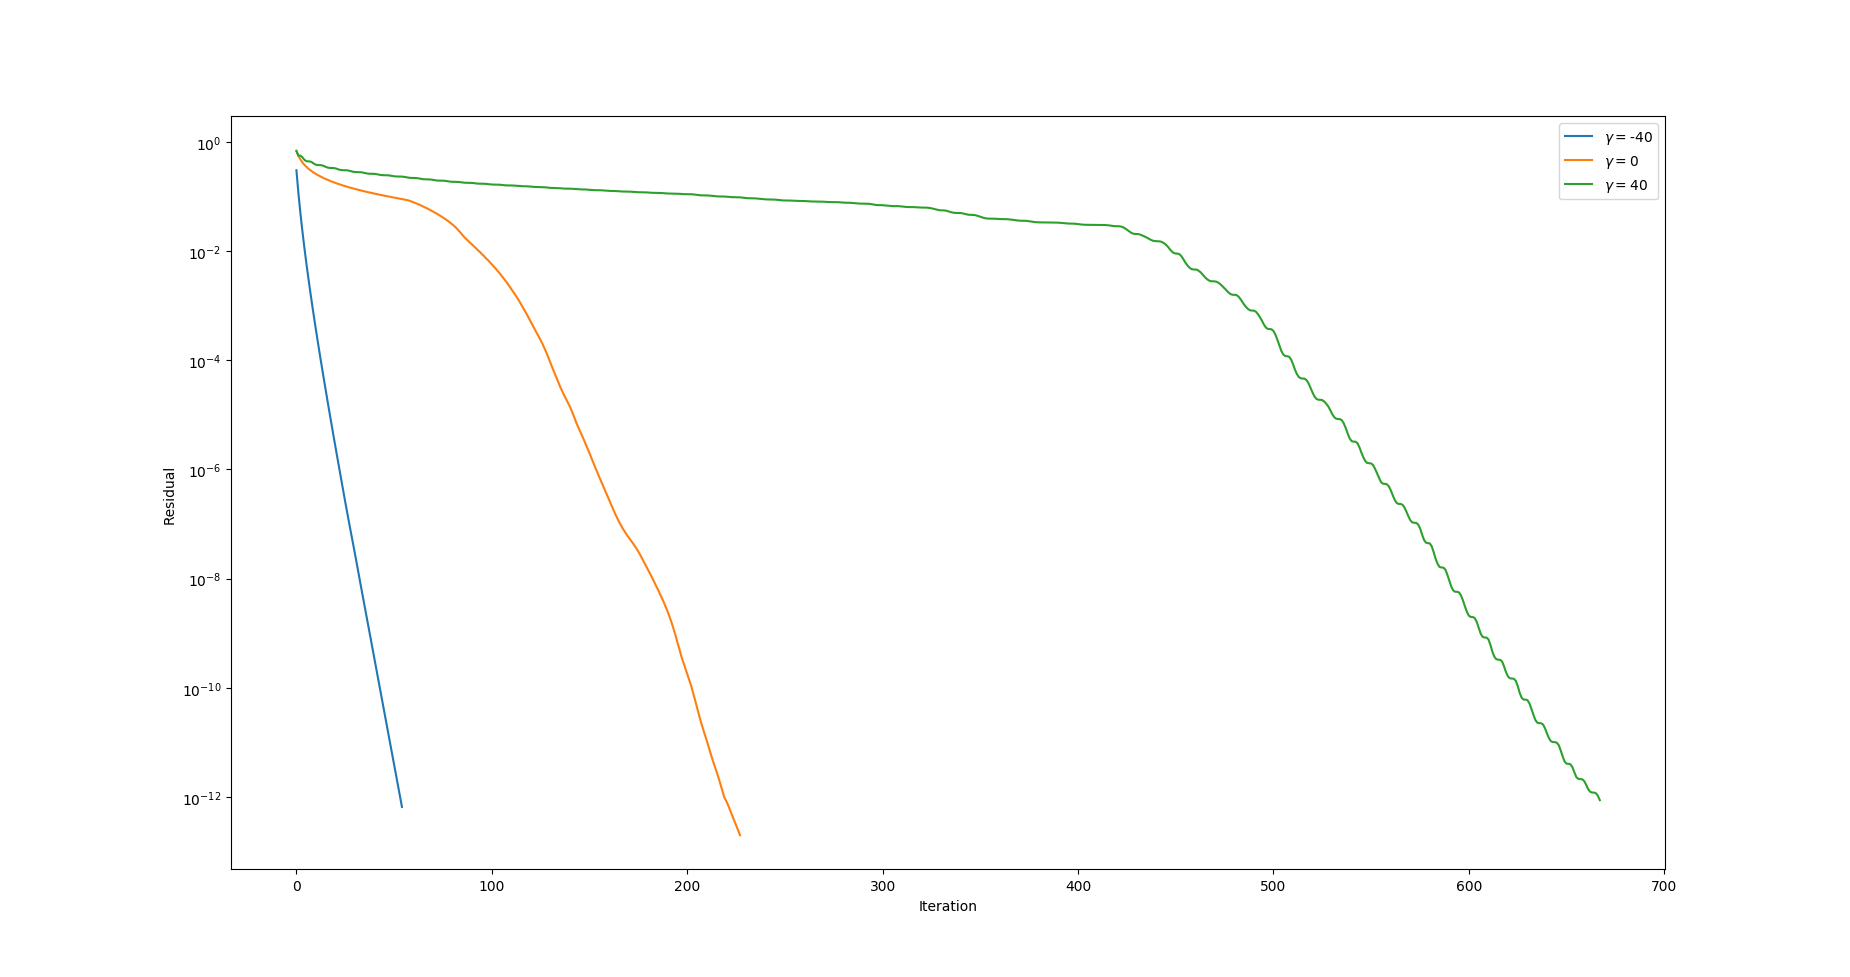
\includegraphics[width=.9\linewidth]{5convergence.png}
	\caption{Convergence history of GMRES for different calues of $\gamma$}
\end{figure}

In order to understand this convergence, the eigenvalues of the discrete equation have to be analyzed. The eigenvalues and eigenvectors of the negative Laplacian are known to be $\lambda_m$ and $\mathbf{x}_m$.
\begin{align}
	L\mathbf{x}_m &= \lambda_m\mathbf{x}_m\\
	\gamma I \mathbf{x}_m &= \gamma \mathbf{x}_m \\
	L\mathbf{x}_m - \gamma I \mathbf{x}_m &= \lambda_m\mathbf{x}_m - \gamma \mathbf{x}_m\\
	\left(L- \gamma I\right) \mathbf{x}_m &= \left(\lambda_m - \gamma\right) \mathbf{x}_m
\end{align}
Thus the eigenvalues of the discrete BVP ($\lambda'$)  are found to be
\begin{equation}
	\lambda'_m = \lambda_m-\gamma
\end{equation}

The eigenvalues of the negative Laplacian are known to be real and are bounded between 0 and the $max(\lambda_m)$.  For $\gamma=40$ there are eigenvalues on both the positive and negative real axis, while for $\gamma=-40$ all eigenvalues are strictly positive, this suggests that GMRES performs best if the discretization matrix is positive definite or negative definite, while it still works reasonably well for semi positive/negative definite matrices, matrices that are neither however take longer to solve with GMRES.
    
\end{document}